\documentclass[11pt,final]{scrbook}
\usepackage[paper=a4paper, twoside, bindingoffset=5mm, headheight=20pt, top=20mm, bottom=40mm,left=25mm,right=35mm]{geometry}
\usepackage[utf8]{inputenc} 	% UTF-8 (Unicode) encoding
%\usepackage{fullpage}
\usepackage{boxedminipage}
\usepackage{varioref}
\usepackage{amsmath,amssymb}    % Mehr Mathe Befehle (z.B. \text{})
\usepackage{minitoc}
\usepackage{graphicx}           % Grafiken einfach einbinden
\usepackage{epstopdf}
%\usepackage[export]{adjustbox}
\usepackage{scrpage2}           % Für Kopfzeilen
\usepackage{tabularx}           % tollere Tabellen
\usepackage{multirow}
\usepackage{booktabs}
\usepackage{array}
\usepackage{units}
\usepackage[squaren, thinspace]{SIunits}
\usepackage{soul} % letter s p a c i n g

% Andere Schriftart als Standard:
% Palatino for rm and math | Helvetica for ss | Courier for tt
\usepackage{mathpazo} % math & rm
\linespread{1.05}        % Palatino needs more leading (space between lines)
\usepackage[scaled]{helvet} % ss
\usepackage{courier} % tt
\normalfont
\usepackage[T1]{fontenc}
\usepackage{subfigure}          % mehrere Graphen in einem
\usepackage{caption}
\usepackage{paralist}

\def\Nabla{\bm{\nabla}}
\def\bm{\mathbf}
\def\curl{\Nabla\times}
\def\div{\Nabla\cdot}
\def\lap{\Delta}
\def\vlap{\Delta}
\def\x{\hat{e}_{x}}
\def\y{\hat{e}_{y}}
\def\z{\hat{e}_{z}}
\def\p{\partial}
\def\h{\hat}
\def\tw{\tilde{\omega}}
\def\gm{\gamma}
\def\om{\omega}
\def\OM{\Omega}
\def\GM{\Gamma}
\def\dw{\delta\omega}
\def\dth{\Delta\theta}
\def\dk{\delta k}
\def\Hdth{\frac{\dth}{2}} %half Delta Theta
\DeclareMathOperator{\Tr}{Tr}

% Alter some LaTeX defaults for better treatment of figures:
% See p.105 of "TeX Unbound" for suggested values.
% See pp. 199-200 of Lamport's "LaTeX" book for details.
%   General parameters, for ALL pages:
\renewcommand{\topfraction}{0.9}	% max fraction of floats at top
\renewcommand{\bottomfraction}{0.8}	% max fraction of floats at bottom
%   Parameters for TEXT pages (not float pages):
\setcounter{topnumber}{2}
\setcounter{bottomnumber}{2}
\setcounter{totalnumber}{4}     % 2 may work better
\setcounter{dbltopnumber}{2}    % for 2-column pages
\renewcommand{\dbltopfraction}{0.9}	% fit big float above 2-col. text
\renewcommand{\textfraction}{0.07}	% allow minimal text w. figs
%   Parameters for FLOAT pages (not text pages):
\renewcommand{\floatpagefraction}{0.7}	% require fuller float pages
% N.B.: floatpagefraction MUST be less than topfraction !!
\renewcommand{\dblfloatpagefraction}{0.7}	% require fuller float pages
\renewcommand{\labelenumi}{\roman{enumi})}

%Farbe
\usepackage{color}
\definecolor{gray}{gray}{0.95}

% Zeilenabstand
\usepackage{setspace}
%\linespread{1.5}
\onehalfspacing

% Code samples
\usepackage{listings}
\lstset{numbers=left, numberstyle=\tiny, numbersep=5pt, stepnumber=1}
\lstset{language=}
\lstset{frame=leftline}
\lstset{basicstyle=\footnotesize\ttfamily, stringstyle=\ttfamily}
\lstset{moredelim=[is][\bfseries]{|*}{*|}}
\lstset{backgroundcolor=\color{gray}}


% Hyperref
\usepackage[square,comma,numbers]{natbib}
\usepackage[pagebackref, pdfborder={0 0 0}]{hyperref}
\renewcommand*{\backref}[1]{}% for backref < 1.33 necessary
\renewcommand*{\backrefalt}[4]{%
	\ifcase #1 % 
		\textit{No citations.}%
	\or
		\textit{Cited on page #2.}%
	\else 
		\textit{Cited on pages #2.}%
	\fi
}%

% last \usepackage
% ============================
% 

% Programmierung von Armin Dobner für Bildunterschriften (slanted)
 \makeatletter
 \renewcommand{\fnum@figure}{{\bfseries \figurename~\thefigure}}
 \renewcommand{\fnum@table}{{\bfseries \tablename~\thetable}}
 \long\def\@makecaption#1#2{%
   \vskip\abovecaptionskip
   \sbox\@tempboxa{#1{\bfseries :} {\slshape #2}}%
   \ifdim \wd\@tempboxa >\hsize
     #1{\bfseries :} {\slshape #2}\par
   \else
     \global \@minipagefalse
     \hb@xt@\hsize{\hfil\box\@tempboxa\hfil}%
   \fi
   \vskip\belowcaptionskip}
 \makeatother



% Absätze
\setlength{\parskip}{1.5ex plus0.3ex minus0.3ex}
\setlength{\parindent}{0pt}

\clubpenalty = 10000
\widowpenalty = 10000

% Kommandos
\newcommand{\code}[1]{{\tt #1}}
\newcommand{\class}[1]{\code{\textbf{#1}}}
\newcommand{\keyword}[1]{\class{#1}}
%\newcommand{\sf}[1]{\textsf{#1}}
%\newcommand{\eqref}[1]{equation~(\ref{#1})}

\renewcommand\ohm{\text{$\Omega$}}
\newcommand{\siox}{SiO$_\text{2}$}

%Konstanten
\newcommand{\Boltz}{k_{\text{B}}}
\newcommand{\psibi}{\psi_{bi}}
\newcommand{\pH}{\text{$p$H}}


% trennung
\hyphenation{dia-me-ter}
\hyphenation{na-no-tu-be}
\hyphenation{na-no-scale}

%Kopfzeile
\pagestyle{scrheadings}
\automark[section]{chapter}
\setlength{\headheight}{3\baselineskip}
\setheadsepline{0.5pt} % Linie oben Zeichnen
\ihead{} %links oben
\chead{}
\lehead{\thepage  \hspace{4em} Chapter \headmark} % rechts oben
\rohead{\headmark \hspace{4em} \thepage}
\ofoot[]{} % Seitenzahl in der Fußzeile entfernen

%\titlehead{\textbf{Technische Universität München \\ Institut für Nanoelektronik \hfill 2011}}
%\title{Carbon Nanotube Thin Film Devices for Biological Sensors}
%\author{Tobias Haeberle}
%\date{\today}

\dedication{To my friends and family.}


% ============================
%  DOCUMENT START
% ============================
\begin{document}

%%
%% Titel-tex
%%
%
%% Die vertikalen Abstände nach Eingabe der Daten bitte selbst anpassen.
  % title page

\begin{titlepage}
%\raggedleft\includegraphics{figures/Universitaet_Logo_RGB.pdf}
\begin{center}
    
\includegraphics[width=\textwidth]{images/Logos2.pdf}% [scale=0.7, right]
    
    \vspace{25mm}	
    
    {
        \scshape	
        Technische Universität München\\
        Fakultät für Elektrotechnik und Informationstechnik\\																										% 
        Professur für Computational Photonics\\
        Prof.Dr.-Ing. Christian Jirauschek
    }
		
    \vspace{25mm}																								

    \begin{LARGE}
        \normalfont\rmfamily \textbf{Coupled Transmission Line/Maxwell-Bloch Equations Approach for Electro-Optical Simulations of Terahertz Quantum Cascade Lasers}\\[6cm]
    \end{LARGE}
   \so{\Large MASTER THESIS}\\[0.5cm]
    
    by Longwei Zhong

    \textbf{May, 2017}\\[2cm]
																	
 																	
\end{center}

\end{titlepage}

\clearpage \thispagestyle{empty} \cleardoublepage 




\pagenumbering{roman}



\chapter*{Abstract}
\addcontentsline{toc}{chapter}{Abstract}
Quantum cascade lasers (QCLs) are compact, electrically pumped semiconductor devices, which are considered to be promising light source for mid-infrared and terahertz radiation. Benefit from this special mechanism they can utilize the electric power more efficiently than other diode lasers and achieve a high output power. Despite its practical significance, generating ultra short pulses from QCLs by mode-locking has achieved only limited success in the past decade. In this work, we studied the influence of external source on the mode-locking of QCLs. A dynamic model based on Maxwell-Bloch equations and transmission line was build to simulate QCLs in time domain. The simulation results were then analyzed and compared with existing experiment results from references to check reliability of the established model.

The purpose of this research is to combine the existing simulation methods and transmission line to build a new model for dynamic modeling of QCLs, which would help to get a better understanding of its theoretical mechanism and redound to search for optimal parameters of mode-locking in experiments. 

\chapter*{Acknowledgements} 
\addcontentsline{toc}{chapter}{Acknowledgements}
I would like to express my deep gratitude to my supervisor Prof. Christian Jirauschek and Mr. Petar Tzenov for their support and constructed criticism during my master thesis project. Especially for Petar, from advance seminar to master thesis, he behaved always modest, professional and patient in my mind. I thank him for being my mentor and friend.

I would like to thank Assistant Professorship of Computational Photonics of TUM, which provides a friendly atmosphere and the opportunity to carry on a research in QCL area. I also want to thank other members in this group Mr. Mark Schmidt and Mr. Michael Riesch. Although we focus on different topics, we had lots of inspiring discussions and I learned a lot from them.

\clearpage
\thispagestyle{empty}

\vspace*{2cm}
\begin{center}
{\normalfont\itshape  I dedicate this work to my beloved mother and father}
\end{center}

%\chapter*{List of Symbols}
%
%
%% ============================
%%  Content
%% ============================
%
%\tableofcontents

\chapter{Introduction}\pagenumbering{arabic}
The operating principle of QCLs was first proposed by R.F. Kazarinov and R.A. Suris in 1971 \cite{kazarinov1971possibility}. However, due to the complexity of fabrication process until 1994 QCLs was firstly demonstrated at Bell Laboratories by Jerome Faist and his colleagues \cite{faist1994quantum}. They have gained considerable attention afterwards. Unlike common semiconductor lasers, which utilize electron-hole recombination to realize electromagnetic radiation, QCLs are unipolar and their emission is based on intersub- band transitions in coupled quantum well superlattices \cite{williams2007terahertz}. Due to lack of suitable radiation sources and detectors this region remains one of the least developed spectral regions. The occurance of QCLs provides a option as a prominent source to help investigate these regions, because their emission wave length as well gain spectrum can be engineered through artificial design \cite{gmachl2002ultra}. To date, only n-type QCLs are successfully realized lasing.  One of the most commonly used material combination for active region is GaAs (well) and $Al_{x}Ga_{1-x}As$ (barrier), where x is the relative amount ration of aluminum to gallium. The intersubband transmission occurs in conduction band, as Fig. shows. Add--> one module of repeated QCL heterostructures!

As a novel type of laser as well as efficient source to generate tera Herz (THz) radiation, THz QCLs showed great potential and have attracted already a lot attentions for developing their possible applications. Compared to X-ray, THz radiation owns relative lower energy ($E=h\nu$), which iwouldn't lead to ionising but still can penetrate many materials (e.g. clothes, paper) except for metals \cite{williams2007terahertz}.  Therefore, it could be used as imaging and sensing for security detection in airport \cite{federici2005thz}, which wouldn't affect the health of our bodies. Another interesting area is astronomy, such as heterodyne receivers \cite{williams2007terahertz}, which requires THz QCLs. Because the radiation from universe is mainly with THz, the research of THz technologies would help to detect and observe those unnoticed radiation from galaxies. 

\section{Background and motivation}
For the past decade since the fist demonstration of QCLs, some groups devoted themselves to improve the operation temperature, up to room temperature has been achieved \cite{bai2011room} through special wells design of QCL structure. Some consisted on generating short pulse with QCLs \cite{wang2009mode}. Active mode-locking was recognized as the only viable route to QCL mode-locking \cite{revin2016active}. The main idea is to lock modes through a modulated injection current with a frequency corresponding to the roundtrip frequency. THz QCLs can be injection locked by modulating a short section of the cavity to open a net gain window with an external RF source. They are biased close to their threshold, while high above threshold pulses are broadened due to multi-mode instabilities (Spatial Hole Burning and Risken-Nummedal-Graham-Haken instability \cite{vukovic2016low}). It was found that mode-locking in THz QCLs is easier than that in mid-infrared \cite{wang2009mode}. Compared with mid-infrared QCLs, the laser transition energy lies below the optical phonon energy, so the upper state of THz QCLs based on bound-to-continuum has generally longer non-radiative relaxation time ($\sim$ 5-10 ps), which makes it easier to realize mode-locking \cite{barbieri2011coherent}. The first successful attempt of mode-locking in THz QCLs was reported in 2010 \cite{gellie2010injection}. By direct amplitude modulation, the mode-locking of a 2.3THz QCL was achieved at 35GHz, which shows locking ranges up to $\sim$225MHz  \cite{gellie2010injection}. Recently, active mode locking of QCLs in an external ring cavity was reported \cite{revin2016active}, which can operate at room temperature. Moreover, benefits from this method, the mode-locking was observed not only at close to the threshold, but also far above it. 

Although there are already those successful experimental attempts by active mode-locking, but a complete theory system is still not available. Different with experimental attempts, theoretical modeling requires more understanding of physical effects and accurate mathematical description as well as assumptions. Due to limited knowledge of unfavorable physical effects and lack of consolidation theory about its mechanism, it has been proven to be difficult to directly employ existing techniques from the ultra fast optics community to realize mode-locking of QCLs, active mode-locking is regarded as a efficient way to achieve it. However, both modulation power and frequency need to be set adequate to get mode-locking. 

Currently, all those simulation methods are based on optical modeling, in which assuming that the applied electrical voltage signal on cavity is constant. But in fact it's not realistic, this electric signal also has wave nature and will propagate along cavity in the same direction as optical field propagation due to the microstrip transmission line structure of QCLs.
\section{Related work}
Accompanied with experimental research, modeling techniques for QCLs are also steady investigated to help get a deep understanding of internal mechanisms and explore unknown effects. Thanks for persistent efforts of researchers, there are already several models as well as solvers which could be used for describing and analyzing various of processes in QCLs, such as density matrix approach \cite{weber2009density}, Maxwell-Bloch equations \cite{gordon2008multimode}, non-equilibrium Green’s function theory \cite{kubis2008non} along with some other modified methods aimed to take more linearities and effects into account. These models have been used, for example, to investigate modulation properties of optical injection-locked QCLs \cite{wang2013rate}, to calculaton for four-level scheme THz QCLs \cite{yasuda2009nonequilibrium}.

However, these exsisting simulation techniques are only able to find solution of steady states rather than dynamic modeling in time domain. A lumped-element approach was proposed in 2007 by Barbieri et al. to investigate amplitude modulation limit \cite{barbieri200713}. After that this concept has been further developed with distributed-parameter transmission-line simulations to quantify injected RF-power to QCLs \cite{maineult2010microwave}. With the aid of a vectorial network analyzer they measured the S-parameters of meta-metal waveguides THz QCLs which were driven under threshold and then extracted distributed parameter from S-parameters. This is the first attempt that by measuring the transmission and reflection coefficients and using transmission-line approach to analyze RF-modulation capabilities of THz QCLs.

\section{Objective}
The objectives of this thesis are as follows:
\begin{enumerate}
\item To build a dynamic model with coupled Maxwell-Bloch equations and  Transmission line method;
\item To verify "pulling effect" in active mode-locking by simulation;
\item To acquire optimal simulation parameters to generate short pulse;
\item To gain a deep understanding of mode-locking behaviors to help QCLs design in the future.
\end{enumerate}


\chapter{Theory}
QCL is composed of a great amount of repeated stacks of heterojunctions, its extreme thin layers (in the order of a few nanometers) of different materials result in the formation of quantum wells and barriers. By solving steady Schroedinger-Poisson equation system, eigenenergies and wave functions of eigenenergies can be determined, which help to design and optimization of QCL structures (e.g. radiation frequency, injection efficiency). Transfer matrix method \cite{jonsson1990solving} and finite-difference method \cite{tan1990self} are efficient methods to help compute numerical solutions of these systems. 
\section{Maxwell-Bloch equations}
As a semi-classical approach, Maxwell-Bloch equations are widely to describe carrier dynamics as well as field dynamics in a laser. Bloch equations are similar with rate equations, but instead of considering scattering rate of laser levels, they model interaction of electrons on different energy levels by using density matrix. For example, a 3-level system is illustrate in Fig. \ref{fig:MB_levelsystem}. As the active region of QCLs consists of periodic structures, for a single period, Bloch equations can be closed by assuming periodic boundary condition $J_{in}=J_{out}$, where J is injection current density.
\begin{figure}[htbp]
\begin{center}
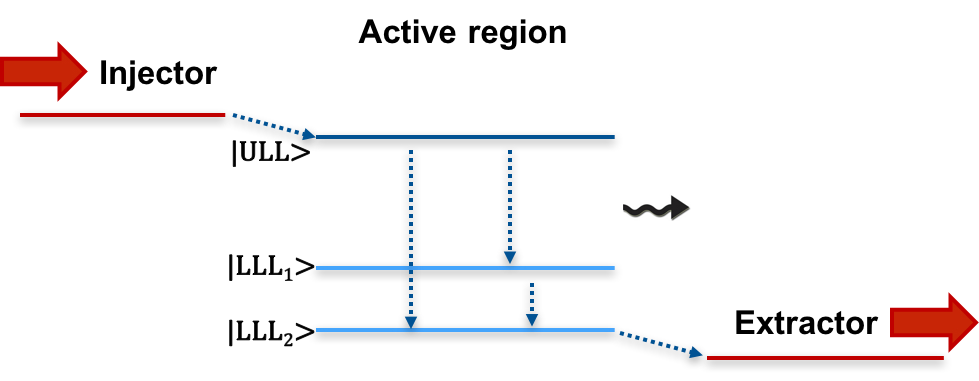
\includegraphics[scale=0.8]{images/MB_levelsystem}
\caption{: Carrier transition in an injector/3-level/extractor system. |ULL> denotes upper laser level and |LLL> is lower laser level. Injector and extractor stand for laser levels in injections region.}
\label{fig:MB_levelsystem}
\end{center}
\end{figure}

Bloch equations are complemented by Maxwell equation or wave equation to include dynamics of electric field (in the direction of propagation). 
\section{Transmission line}
Transmission line model was created by Oliver Heaviside \cite{heaviside2008electromagnetic} and usually consists of two separated conductors and medium in between (Fig. \ref{fig:TLcircuit}). The conventional TLM is based on Telegrapher's equations (\ref{eq:TLequation1})(\ref{eq:TLequation2}), which describe the evolution of voltage and current both spacial and temporal on an electrical transmission line. These two differential equations contains four distributed components (R', L', G', C') which vary from different transmission lines: R' is distributed resistance of conductors, which is represented by a series resistor in ohms per unit length ($\Omega /m$); L' is distributed inductance resulting from the magnetic field around the line due to self-inductance, which is represented by a series inductor in henries per unit length ($H/m$); G' is distributed conductance of the dielectric material separating the two conductors, which is expressed in siemens per unit length ($S/m$) and represented by a shunt resistor with resistance of 1/G'; C' is distributed capacitance of transmission line, which is represented by a shunt conductor in farads per unit length ($F/m$).
% TL equivalent circuit figure
\begin{figure}[htbp]
\begin{center}
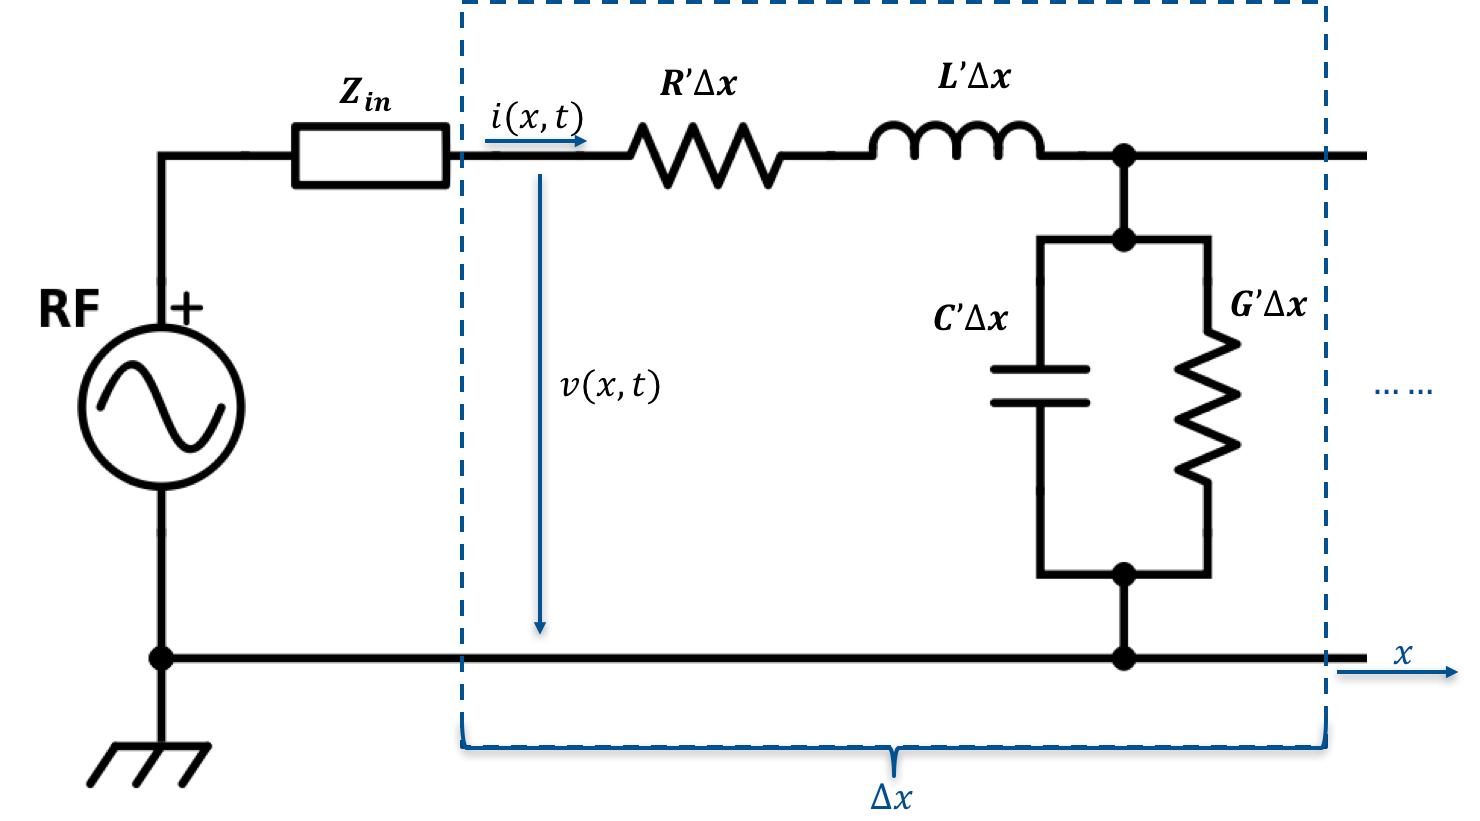
\includegraphics[scale=0.4]{images/TLcircuit}
\caption{: Schematic representation of the elementary component of a transmission line. $Z_{in}$ denotes wire impedance.}
\label{fig:TLcircuit}
\end{center}
\end{figure}

Transmission line can be further classified in lossy/non-lossy transmission line and uniform/nonuniform transmission line with regarding to characteristics of its conductors and medium. When no resistance (conductor) and conductance (dielectric medium) exist, it can be regarded as ideal transmission line which contains only L' and G'. In uniform transmission line all those distributed components are uniformly distributed along line. Therefore, under the assumptions above and considering the conductance of active region, the simulated QCL can be defined as a one-dimensional (1D) nonlinear non-uniform lossy transmission line, which is more complex than common transmission line problems.

% Transmission line equations
Telegrapher's equations:
\begin{eqnarray}
\frac { \partial v(x,t) }{ \partial x }  &=& -L'\frac { \partial i(x,t) }{ \partial t }-R'i(x,t) \label{eq:TLequation1}\\
\frac { \partial i(x,t) }{ \partial x }  &=& - C'\frac { \partial v(x,t) }{ \partial t }-G'v(x,t) \label{eq:TLequation2}
\end{eqnarray}

\section{Mode-locking}
Light generated by lasers owns high coherent compared with from other light sources. Nevertheless, it has still large bandwidth of optical gain, the modes inside cavity osculate independently and don't have fix phase, which leads to wide pulse. By uncertainty principle, if pulse duration is quite short, its bandwidth muss be larger. For example, for a Gaussian shape pulse the minimum possible pulse duration $\Delta t$ can be calculated with
\begin{equation}
\Delta t=\frac{0.441}{N\Delta \nu}.
\end{equation}
Where 0.441 is pulse shape dependent time bandwidth product, which for a hyperbolic-secant-squared pulse shape is 0.315. N and $\Delta \nu$ is amount of modes and bandwidth of pulse, respectively. This formula above could be be used for roughly evaluating the shortest possible pulse width. However, in real case, many other factors have to be taken into consideration, such as dispersion of the cavity, pulse shape and so on.

Mode-locking is a technique in optics, which locks multi-mode in resonant laser cavity by enforcing coherence between modes to produce extra short pulse\cite{haus2000mode}. Methods of mode-locking can be simply classified as active mode-locking (AML) and passive mode-locking(PML) depending on whether it is induced by itself (e.g. absorber) or requires external source (e.g. RF source).

For active mode-locking, ideally the modulation frequency is exactly at $ f_{tr}$, but even if modulated at frequency of a little variation with $ f_{tr}$, the laser could still be mode-locked, the maximal possible frequency interval is called locking range.
\chapter{Model}
The dynamic model consists of two parts. One of them is optical modeling, which is used for describing the carrier transition  as well as light propagation inside cavity (microcosmic). The other is based on transmission line to obtain voltage and current distribution along cavity (microcosmic). Although each of them has separate solver, both will be simulated simultaneously and can affect with each other.
\section{Optical modeling}
Similar with the existing modeling methods, in this model light propagation is described with Maxwell' equation while carrier transition is determined by Bloch equation. Without regard to lateral non-uniform distribution at boundaries \cite{huang2014non, dhar2015nanoscopic} QCL can be simplified to 1D structure in the direction of propagation (x axis), which means the electrical components were uniformly distributed throughout the cross-sectional area. 

\subsection{Carrier transition}
To simulate active region of QCLs, the density matrix model from Ref. [cite Belyanin] was applied to include total of four subband levels, and more importantly to allow all relevant system parameters, such as the eigenenergies, dipole moments and all scattering rates to be bias dependent. 

As a prototypical QCL design, the sub-band structure configuration illustrated in Fig. \ref{fig:4Levels}, consists of 4 relevant levels per period, i.e. levels from 1 to 4, where level 4 denotes the upper laser state, level 3 the lower laser level, level 2 is an extraction level which eases the electron extraction from 3, and finally level 1 denotes the depopulation level of the period, which also coincides with the injector state (1') of the next module. 

\begin{figure}[htbp]
\begin{center}
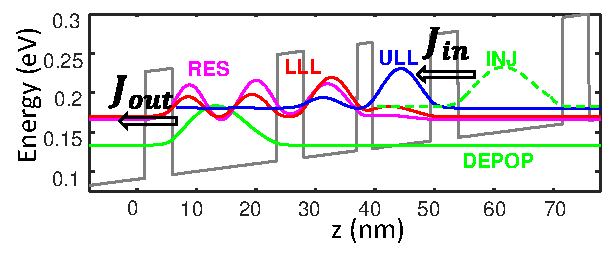
\includegraphics[scale=1.2]{images/WFs.pdf}
\caption{Sub-band structure configuration of QCL.}
\label{fig:4Levels}
\end{center}
\end{figure}

The time evolution of the density matrix is given by the von Neumann equation, which was coupled with a wave equation. $E_z(x,t)$ denotes the $z$-component of electric field (and also the assumed laser growth direction).  
\begin{subequations}
	\label{eq:dmequations}
 \begin{align}
	\frac{d\rho_{44}}{dt} &= J +i\frac{ez_{43}}{\hbar}E_z(\rho_{43}-\rho_{34}) + \sum_{j\neq 4} \frac{\rho_{jj}}{\tau_{j\rightarrow 4}}  - \frac{\rho_{44}}{\tau_{4}}, \\
	\frac{d\rho_{33}}{dt} &= -i\frac{ez_{43}}{\hbar}E_z(\rho_{43}-\rho_{34}) + \sum_{j\neq 3} \frac{\rho_{jj}}{\tau_{j\rightarrow 3}} - \frac{\rho_{33}}{\tau_{3}}, \\
	\frac{d\rho_{22}}{dt} &= \sum_{j\neq 2} \frac{\rho_{jj}}{\tau_{j\rightarrow 2}} - \frac{\rho_{22}}{\tau_{2}}, \\
	\frac{d\rho_{11}}{dt} &=  -J + \sum_{j\neq 1} \frac{\rho_{jj}}{\tau_{j\rightarrow 1}} - \frac{\rho_{11}}{\tau_{1}}, \\
	\frac{d\rho_{43}}{dt} &= - i\omega_{43}\rho_{43} + i\frac{ez_{43}}{\hbar}E_z(\rho_{44}-\rho_{33})-\Gamma_{\parallel 43}\rho_{43}.
 \end{align}
\end{subequations}
In Eqn. (\ref{eq:dmequations}) $\rho_{ij}$ denotes the $ij-$th density matrix element,  $z_{43}$ the optical transition's dipole moment, $e$ the elementary charge, $\hbar$ is the reduced Plank's constant. Also the parameter $1/\tau_{i\rightarrow j}$ is the net scattering rate from level $i$ to level $j$, calculated by our ensemble Monte Carlo code and incorporating, amongst others, longitudinal optical (LO) phonon, interface roughness and electron electron scattering mechanisms [cite]. Lastly $1/\tau_{i} = \sum_j 1/\tau_{i\rightarrow j}$ is the inverse lifetime of level $i$ and $\Gamma_{\parallel 43} = (\tau_4+\tau_3)/(2\tau_4\tau_3)+1/\tau^*$ is the dephasing rate of the optical transition, including lifetime broadening and a phenomenological pure dephasing $1/\tau^*$ rate due to intrasubband scattering processes [cite ANDO model]. The only scattering mechanism treated quantum mechanically is the optical transition between the upper and lower laser states. One can also fully coherently include resonant tunneling between the injector 1' and the upper laser state 4, which leads to a modified system of equations with larger number of independent variables and is thus more computationally demanding [cite]. Furthermore such an approach does not allow for the inclusion (without $k-$space discretization) of second order tunneling current into the simulations, which has been shown to be the origin of negative the differential conductivity and dispersive gain in quantum cascade lasers []. 

In the tight-binding basis [cite], we can assume that the only electron transport channel across the QCL periods is via the resonant tunneling current between the injector and the upper laser state. When second order scattering effects are considered, under a few relaxing approximations, this tunneling current is given by [cite Terrazzi]
\begin{align}
\label{eq:current}
J &= en^s\frac{\Omega_{AC}^22\Gamma_{\parallel 1'4}}{\epsilon^2+4\Gamma_{\parallel 1'4}^2}\Big\{\Theta(\epsilon)(\rho_{11}-\rho_{44}e^{-|\hbar\epsilon|/k_BT}) \nonumber \\
&+\Theta(-\epsilon)(\rho_{11}e^{-|\hbar\epsilon|/k_BT}-\rho_{44})\Big\}.
\end{align}
In Eqn. (\ref{eq:current}) $n^s$ denotes the sheet carrier density, $\Theta(\cdot)$ is the Heaviside function and the term $e^{-|\hbar\epsilon|/k_BT}$ denotes an effective "weight" factor modeling the assumption of thermalized $k$-space distribution of the injector and upper laser level electrons with the same thermal energy $k_BT$ in each subband.   

\subsection{Light propagation}
The wave equation inside cavity can be described by the following equation with assumption of weak nonlinearity and inhomogeneity
\begin{align}
\label{eq:waveqn}
\left [\frac{c^2}{n_{THz}^2} \frac{\p^2}{\p x^2} -\frac{\p^2}{\p t^2} \right ] E_z =\frac{1}{\epsilon_0 n_{THz}^2}\frac{\p^2}{\p t^2}P,
\end{align}
where  $n_{THz}$ denotes the background refractive index of the bulk active region, $c$ is the velocity of light in vacuum and $\epsilon_0$ is the permittivity of free space. The symbol $P$ denotes the (nonlinear) polarization of the two level system and is given by 
\begin{equation}
P(x,t) =  -\frac{n^s}{L_p}\Gamma ez_{43} (\rho_{43}+\rho_{34}),  
\end{equation}
with $\Gamma$ is the field confinement factor and $L_p$ is the period length. 

For the final set of equations, the rotating wave and slowly varying envelope approximations [cite] are employed in order to reduce the wave equation (\ref{eq:waveqn}) to a pair of propagation equations, an fast oscillating terms from the density matrix equations (\ref{eq:dmequations}) was eliminated as well. The corresponding final formulas are slightly modified versions of those in [cite me, cite belyanin], and therefore we omit them here for brevity. Besides, in all subsequent calculations, the effect of the inversion grating on to the current density has been taken into consideration, in an analogous manner to [cite belyanin]. 

\section{Electrical modeling}
In the electrical modeling, a modified Transmission Line Method (TLM) was introduced in order to realize a dynamic modeling in time domain. TLM is a very efficient methode which is already widely used for evaluation and dynamic modeling especially in high frequency region where wave nature muss be taken into accout, for example, contact resistance extraction in organic field- effect transistors \cite{xu2010modified}, dynamic modeling of flow in pipelines \cite{johnston2014enhanced} etc. However, in QCLs are transverse magnetic (TM) modes \cite{yan2009directional} while TLM is specially for analysis of transverse electromagnetic (TEM) modes, in which neither electric nor magnetic field in the direction of propagation. The common used metal-metal waveguide (microstrip structure) in QCLs can be regarded as quasi-TEM structure, as the substrate ($ \sim $ 10 um) is quite thin in terms of wavelength (30 mm $ \sim $ 300 mm), and the width of strip conductor is very narrow ($ \sim $ 50 um) in terms of wavelength as well, therefore, a static analysis should be still perfectly adequate in this case.

\begin{figure}[htbp]
\begin{center}
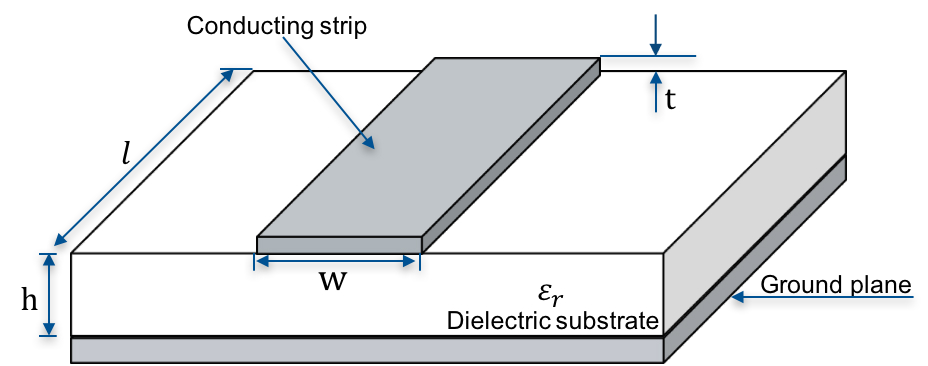
\includegraphics[scale=0.8]{images/Microstrip.pdf}
\caption{Microstrip structure.}
\label{fig:Microstrip}
\end{center}
\end{figure}

\subsection{Transmission line approach}
In this model, the vertical current component resulting from conductance of active region (n-doped semiconductor) under bias is calculated by current density J'(x,t) rather than by distributed conductance G'. Current density J(x,t) is nonuniform and bias dependent, it will be obtained by carrier transmission in optical part. Furthermore, although $v(x,t)$ and $i(x,t)$ in Eqn. (\ref{eq:TLequation1}) and (\ref{eq:TLequation2}) are special for high frequency signal, they will be still valid if the transmission line was supplied additionally with a dc source. Therefore, the Telegrapher equations will be modified as following:

\begin{eqnarray}
\frac { \partial V(x,t) }{ \partial x }  &=& -L'\frac { \partial I(x,t) }{ \partial t }-R'\tilde i(x,t) \label{eq:TLequation5}\\
\frac { \partial I(x,t) }{ \partial x }  &=& - C'\frac { \partial V(x,t) }{ \partial t }-wJ(x,t). \label{eq:TLequation6}
\end{eqnarray}
where V(x,t) and I(x,t) are voltage and current signal at a node x. 
\subsubsection{Boundary conditions}
Boundary conditions account for the completeness of differential equations at the boundary. In order to refine the boudaries and avoid hard variation of electrical components, a cascading of $\pi$ networks\cite{orlandi1996fdtd} is introduced for the distributed transmission line by splitting the shunt capacitance and conductance in half with two parallel capacitors and conductors at boundary, which is illustrate in Fig. \ref{fig:BoundaryCondition}. 

In active mode-locking, QCL is supplied with source $ {V}_{S} $ which consists of a DC voltage source $ {V}_{DC} $ and an external RF source $ {V}_{RF} $. These two sources are combined through bias-T and the source voltage can be expressed with $ {V}_{S}=V_{DC}+{V}_{RF} $. Due to existence of wire impedance there will be voltage drop on it, so the voltage at node 0 is not equal to source voltage $ {V}_{S} $.
% Boundary condition figure
\begin{figure}[htbp]
\begin{center}
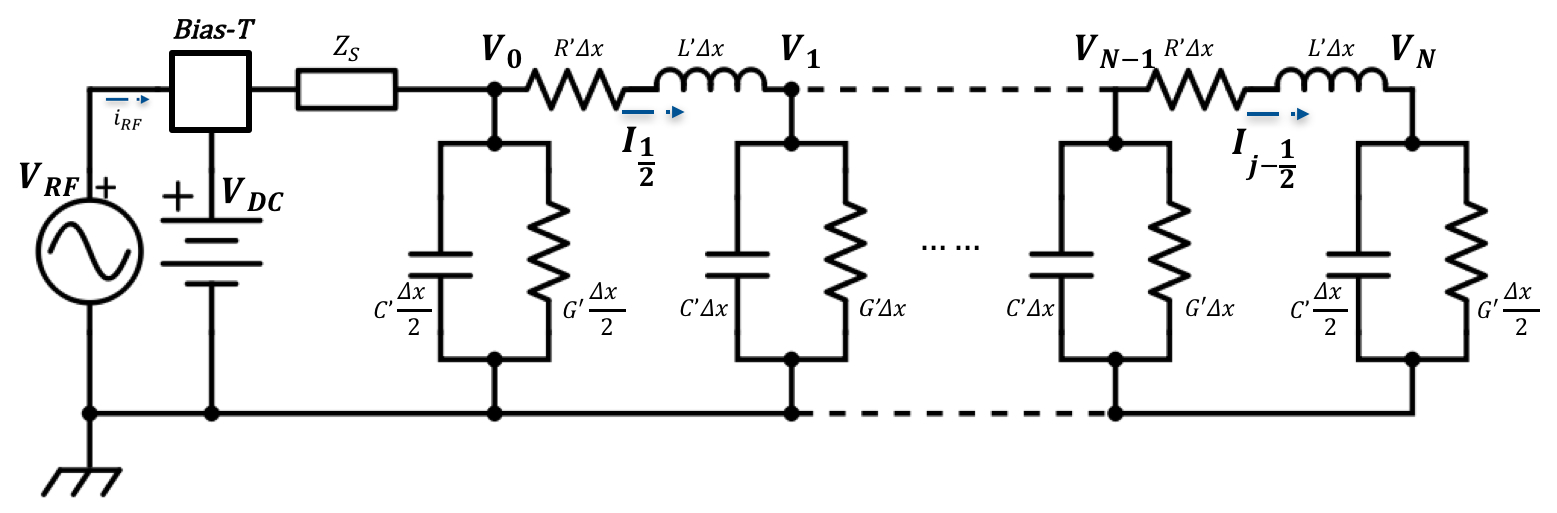
\includegraphics[scale=0.6]{images/pi_representation.pdf}
\caption{Schematic of cascade $\pi$ network representation and Thévenin equivalent circuit. }
\label{fig:BoundaryCondition}
\end{center}
\end{figure}

By using Kirchhoff's voltage law (KVL), 
\begin{equation}
V_{S}^{n}={ V }_{ RF }^{n}+{V}_{DC} = {Z}_{S}\widetilde{ i }_{ S }^{ n } + {V}_{0}^{n} \label{eq:Vs_n}
\end{equation}
where $\widetilde{ i }_{ S }^{ n }$ denotes ac component among whole current between bias-T and QCL. RF source has wave function of $V_{RF}^{n}=M_{A}\cos(2\pi f_{RF}n\Delta t)$, where $M_{A}$ stands for modulation amplitude. 

As the right side of QCL lefts open, no current component exists at the end node. Consequently, the boundary condition for current is set as $I_{N+\frac{1}{2}}^{n}=0$.
%\begin{equation}
%{ V }_{ 0 }^{ n+\frac{3}{2} }=\frac{2Z_{S}C'\Delta x}{Z_{S}C'\Delta x+\Delta t}{ V }_{ 0 }^{ n+\frac{1}{2} }+\frac{ \Delta t-Z_{S}C'\Delta x }{Z_{S}C'\Delta x+\Delta t}{ V }_{ 0 }^{ n-\frac{1}{2} }+\frac{2\Delta t}{Z_{S}C'\Delta x+\Delta t}\big [{ V }_{ RF }^{ n+1 }-V_{ RF }^{ n }...
%\end{equation}
%\hspace{7cm}$- Z_{S}\big ({ I }_{ \frac { 1 }{ 2 }  }^{ n+1 }-{ I }_{ \frac { 1 }{ 2 }  }^{ n }+w\frac { \Delta x }{ 4 }(J_{0}^{n+\frac{3}{2}}-J_{0}^{n-\frac{1}{2}})\big )\big ]$


%OR:$********************************************$
%
%Use 40 GHz low loss RF coaxial cable which has 50 Ohms impedance.
%
%$Z_{S}=\sqrt{\frac{L}{C}}=50\Omega$ (C = 27 pF/ft, L = 6.75e4 pH/ft, one foot length, 1 foot = 0.3048 m)
%
%By using Kirchhoff's law, 
%\begin{eqnarray}
%{ V }_{ S }^{n+\frac{1}{2}}-{V}_{0}^{n+\frac{1}{2}} = L\frac{d{I}_{S}^{n+\frac{1}{2}}}{d{t}}\\\label{eq:BC_1}
%{ I }_{ S }^{n+\frac{1}{2}} = { I }_{ \frac{1}{2}}^{n+\frac{1}{2}}+C\frac{d{V}_{0}^{n+\frac{1}{2}}}{d{t}}\label{eq:BC_2}
%\end{eqnarray}
%where ${ I }_{ S}$ denotes whole current from source after bias-T, which is relevant to current transmission from both RF and DC source. However, that cannot be directly obtained through iterative process. Substitute Eqn. \ref{eq:BC_2} to \ref{eq:BC_1}, leading to:
%\begin{eqnarray}
%{ V }_{ S }^{n+\frac{1}{2}}-{V}_{0}^{n+\frac{1}{2}} &=& L\frac{d{I}_{\frac{1}{2}}^{n+\frac{1}{2}}}{d{t}}+LC\frac{d^{2}{V}_{0}^{n+\frac{1}{2}}}{ dt^{2}}\\
%&=& L\frac{{I}_{\frac{1}{2}}^{n+1}-{I}_{\frac{1}{2}}^{n}}{\Delta t}+LC\frac{{V}_{0}^{n+\frac{3}{2}}-2{V}_{0}^{n+\frac{1}{2}}+{V}_{0}^{n-\frac{1}{2}}}{(\Delta t)^{2}}
%\end{eqnarray}
%Then the equation above is rearranged to get an explicit update expression at boundary:
%\begin{equation}
%{ V }_{ 0 }^{ n+\frac{3}{2} } = (2-\frac{(\Delta t)^{2}}{LC}){ V }_{ 0 }^{ n+\frac{1}{2} }-{ V }_{ 0 }^{ n-\frac{1}{2} }+\frac{(\Delta t)^{2}}{LC}[V_{S}^{n+\frac{1}{2}}-\frac{L}{\Delta t}({I}_{\frac{1}{2}}^{n+1}-{I}_{\frac{1}{2}}^{n})]
%\end{equation}


\subsubsection{Initial conditions}
Adequate initial conditions play a important role as well to acquire an accurate solution. However, real initial conditions for electrical distribution are not possible to be determined and verified. They can be only analytically set, which means a reasonable station at very beginning. In this case, supposing that QCL was biased by DC source barely at t$\leqslant 0$, no RF signal has arrived and no lasing yet. The following initial conditions are defined:
\begin{eqnarray}
V_{0}^{0} &=& V_{1}^{0} =...=V_{j}^{0}...=V_{N}^{0} = V_{DC}\\
I_{S}^{0}&=&\int _{ \Delta x/2 }^{ L-\Delta x/2 }{ wJ(x,0)dx+ } w\frac { \Delta x }{ 2 } (J_{ 0 }^{ 0 }+J_{ N }^{ 0 })\label{Eqn. Is}\\
I_{j+\frac{1}{2}}^{0} &=& [I_{S}^{0}-w\frac{\Delta x}{2}(J_{0}^{0}+J_{N}^{0})]\times \frac{N-1-j}{N-1}+w\frac{\Delta x}{2}J_{N}^{0} \hspace{3mm} (j=0,1...,N-2)\\
I_{N-\frac{1}{2}}^{0}&=&w\frac{\Delta x}{2}J_{N}^{0},
\end{eqnarray}
where, $I_{S}^{0}$ is the initial current injection, which can be obtained by integrating J(x,0) over x from optical model. N is the number of the last node while j integer ranging from 0 to N-2. The initial condition for current is under assumption that at very beginning the current was linearly distributed along active region in x direction.

\subsection{Distributed components}
The involvement of transmission line requires distributed component parameters. Except for distributed conductance G', which will be calculated in optical part, distributed resistance R', distributed inductance L' as well as distributed capacitance C' still need to be determined. They can be either calcuted as convertial passive components (plane resistor, parallel plane capacitor and inductor), or extracted from S-Parameter, which can be directly measured with network analyser. The former methode is simple and also don't require any extra tests, but could lead to large error due to neglection of fringe effect\cite{pillai1970fringing} as well as high frequency influence. The latter is based on experiments, so shows higher accuracy compared with former, but requires extra experiments as well as equipment, which is not always feasible for simulation research. In this work, these parameters of distributed components were eliminated by simple physical calculation assuming that device is with infinite length.

\subsubsection{Distributed capacitance}
Numerically, one only have to consider a small, bounded 2D region with assumption of uniform cross-section going into the page (See Fig. \ref{fig:Gauss2D}). The strip potential was set to 1 V while the boundary to 0 V.  Between strip line and boundary (box) there is no charges, therefore, the electric potential inside the box can be solved. According to Gauss's law in 2D, the surface charge quantity (colon per unit length) can be calculated by integrating the surrounding electric field of strip over arbitrary closed path $l$ with equation
\begin{eqnarray}
\frac { { \partial  }^{ 2 }\phi  }{ \partial { y }^{ 2 } } &+&\frac { { \partial  }^{ 2 }\phi  }{ \partial { z }^{ 2 } } =0 \label{Eqn:TL_C(2)}\\
{ Q }_{ S }&=&\oint _{ l }{\varepsilon_{0}\varepsilon_{r}\overrightarrow { E } \cdot d\overrightarrow { r } },
\end{eqnarray}
where $\varepsilon_{0}$ is permittivity in free space and $\varepsilon_{r}$ is relative permittivity of medium, which in this case are air ($\epsilon_{r}\approx 1$) and semiconductor (active region of QCL, $\epsilon_{r}\approx 12.96$). Here a rectangular was chosen as integration path for the sake of simplification. Then the distributed capacitance $C'=\frac{Q_{S}}{\phi}$.

\begin{figure}[htbp]
\begin{center}
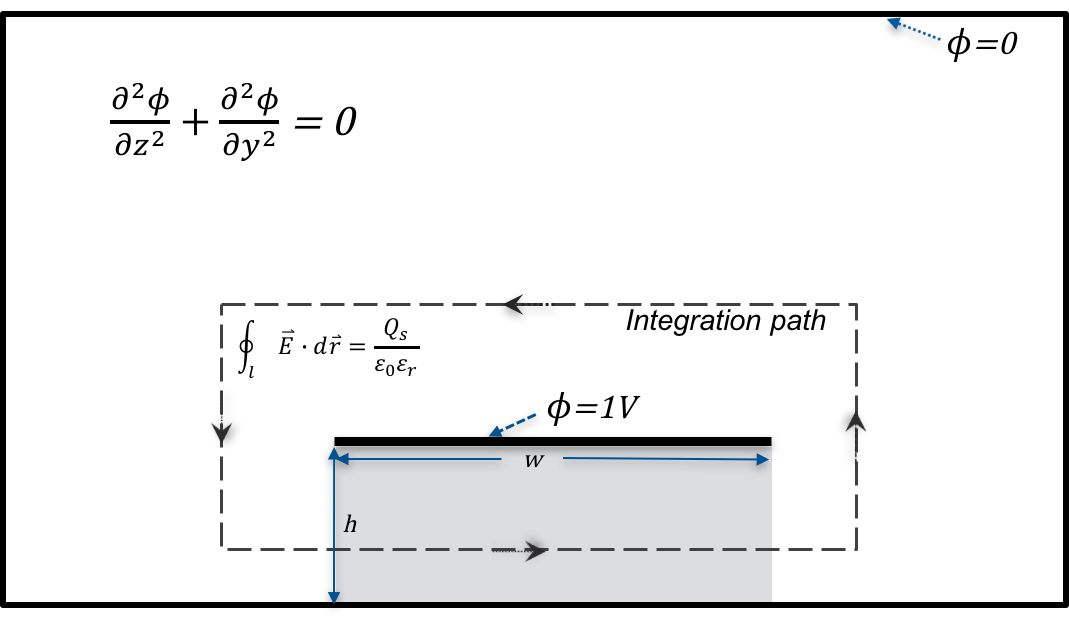
\includegraphics[scale=0.5]{images/Gauss2D.pdf}
\caption{Gauss's 2D equation.}
\label{fig:Gauss2D}
\end{center}
\end{figure}

\subsubsection{Distributed inductance}
In order to evaluate the self-inductance of surface metal layer in QCLs, Biot–Savart law \cite{grant2013electromagnetism} is used for computing resultant magnetic field $\textbf{B}$ (SI unit: Tesla) at surrounding which is generated by a steady current $\textbf{I}$. The distributed inductance L' is inhere characteristic for a certain metal or wire, and is independent of applied current value.
 \begin{figure}[htbp]
\begin{center}
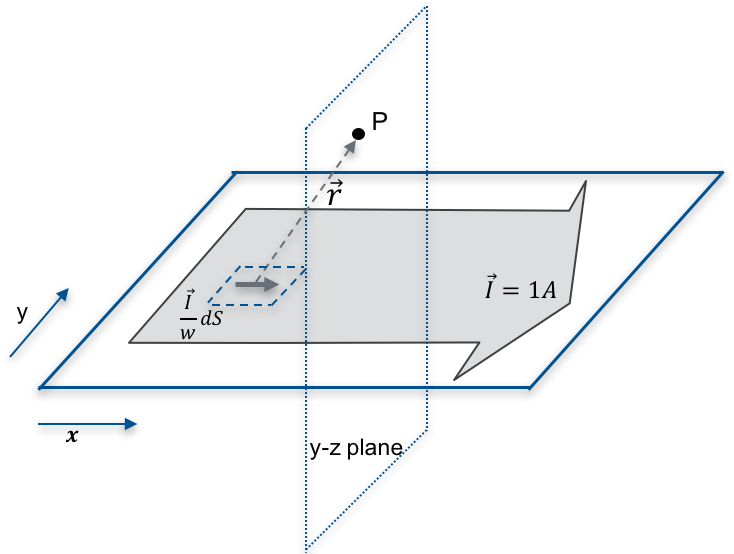
\includegraphics[scale=0.9]{images/TL_L(2).pdf}
\caption{The vector $\vec{ r } $ pointing from the surface element to the observation point.}
\label{fig:TL_L(2)}
\end{center}
\end{figure}

\begin{equation}
\textbf{B}=\frac{\mu_{0}}{4\pi}\int _{ C }{ \frac { Id\textbf{l}\times \textbf{r} }{ |\textbf{r}| ^{3}}}
\end{equation}
where $\textbf{l}$ is the current unit length and $\textbf{r}$ is the displacement vector from current unit to the computed point, C is the path that current flows. Boldface denotes that symbols are vector quantities.

In QCLs with metal-metal structure, the thickness of top metal is usually extremely thin which is around 80 nm ($8\times 10^{-8} m$). Therefore, it can be regarded as a current sheet with assumption of no thickness (See Fig. \ref{fig:TL_L(2)}). The magnetic field resulting from a current unit is $d\textbf{B}_{P}=\frac { \mu \textbf{I}\times { \textbf{r}}dS }{ 4\pi w{ r }^{ 3 }}$ while the magnetic field at a point $ \textbf{B}_{P}$ results from the magnetic field of each current unit. Hence, it can be evaluated by adding all these together with superposition principle:
\begin{equation}
 \textbf{B}_{P}=\int _{ -\frac { w }{ 2 }  }^{ \frac { w }{ 2 }  }{ \int _{ -\frac { l }{ 2 }  }^{ \frac { l }{ 2 }  }{ { \frac { \mu { \textbf{I} }\times { { \textbf{r} } }_{ i,j } }{ 4\pi w{ r }_{ i,j }^{ 3 } }  } }  } dxdy
\end{equation}

Similar with in estimation of distributed capacitance, assuming the cavity has infinite length, the formula above can be simplified by its 2D version 
\begin{equation}
 \textbf{B}_{P}=\int _{ -\frac { w }{ 2 }  }^{ \frac { w }{ 2 }  }{ { \frac { \mu { \textbf{I} }\times { { \textbf{r} } }_{ i } }{ 2\pi w{ r }_{ i,j }^{ 2 } }  }}  dy. \label{Eqn.:TL_L(2)}
\end{equation}
Then magnetic flux $\Phi$ can be calculated by integrating $ \textbf{B}_{P}$ over a closed path. So the distributed inductance can be estimated in this way $L'=\frac{\Phi }{I}$.
\subsubsection{Distributed resistance}
Distributed resistance is frequency dependent and can not be roughly estimately by using similar method as above. But it can be easily obtained by measuring the S-parameter of QCL \cite{maineult2010microwave}, which shows constant value when under certain frequency $ R'=4.5\times10^{-5}\sqrt{f_{RF}}$  $\Omega/mm$ \citep{maineult2010microwave}. The top metal layer of their QCL is similar with in this work, therefore, this relationship between distributed resistance and frequency will be still suitable to be applied in this simulation.
%\begin{equation}
%R=\frac{1}{2(w+t)}\sqrt{\frac{\pi \mu f_{RF} }{\sigma}}
%\end{equation}
%where, $t$ is the thickness of top conductor, $\mu$ and $\sigma$ is the magnetic permeability coefficient and conductivity, respectively. The equation above is obtained by considering the skin effect

\chapter{Numerical Treatment}
\section{Discretization}
Following Yee’s staggered grid approximation\cite{yee1966numerical}, voltage and current are discretized with separation of $\Delta x/2$ and $\Delta t/2$ in space and time respectively (See Figure \ref{fig:Discretisation}), which leads to a second-order accurate approximation. Voltage V(x,t) and current I(x,t) samples are then expressed as $ V\big(j\Delta x, (n+\frac{1}{2})\Delta t\big)$ and $ I\big((j+\frac{1}{2})\Delta x, n\Delta t\big)$, where j and n are integers. For reasons of simplicity, in the following text they will be replaced by $ V _{ j }^{ n+\frac{1}{2}}$ and ${ I }_{ j+\frac{1}{2} }^{ n }$. After discretization, the first-order derivative of voltage $\partial V(x,t)$ as well as current $\partial I(x,t)$ in space and time can be simply calculated with central difference method\cite{yang2012central}. 
% Discretisation figure
\begin{figure}[htbp]
\begin{center}
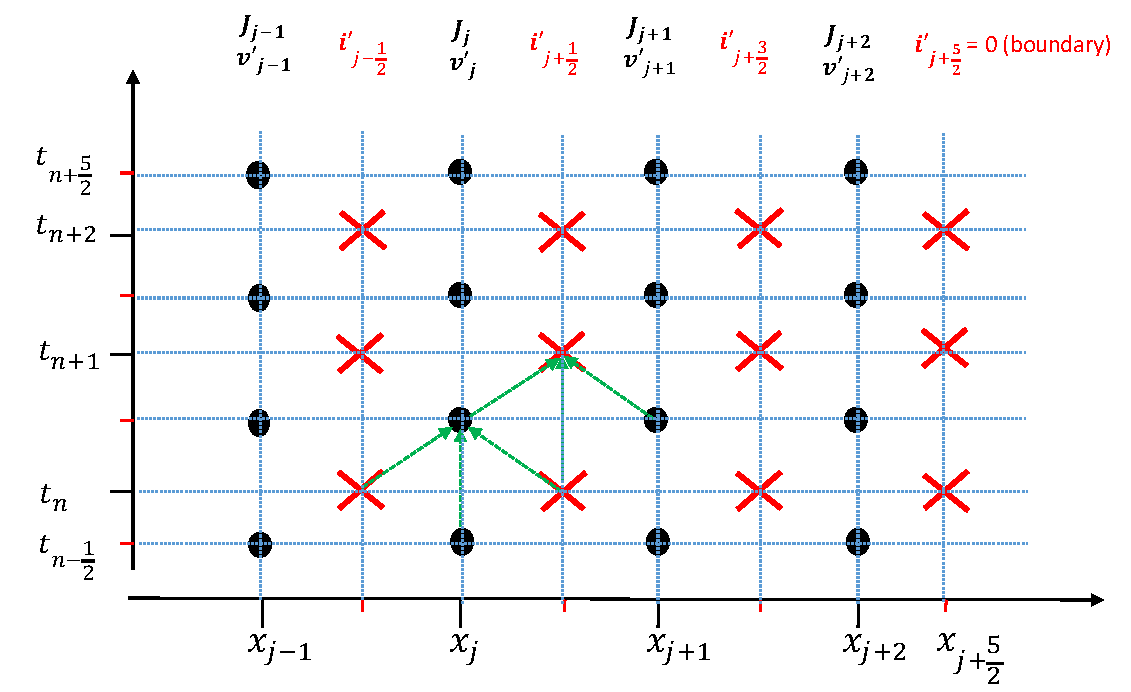
\includegraphics[scale=0.6]{images/Discretization}
\caption{Discretization along a staggered temporal and spatial grid.}
\label{fig:Discretisation}
\end{center}
\end{figure}

In order to solve these two partial differential equations, finite difference in time domain (FDTD) method is applied which owns second order accuracy. Theoretically the smaller these step values were set, the more accurate their solution will be. But in real computation it wouldn't be chosen unlimited small. Therefore, "magic time step" \cite{li1992simulation} is chosen with regarding to stability, which is expressed as
\begin{equation}
\Delta t=n\Delta x/c_{0}=n\sqrt{\varepsilon_{0}\mu_{0}}\Delta x,
\end{equation}
where n is the refractive index of active region, which was set 3.6 for THz in this work.

\subsubsection{Transmission line equations}
Subsequently, the original Telegrapher's equations (\ref{eq:TLequation1}) and (\ref{eq:TLequation2}) are constructed as:
\begin{eqnarray}
\frac { { V }_{ j+1 }^{ n+\frac{1}{2} }-{ V }_{ j }^{ n+\frac{1}{2} } }{ \Delta x } & \approx & -L'\frac { { I }_{ j+\frac{1}{2} }^{ n+1 }-{ I }_{ j+\frac{1}{2} }^{ n } }{ \Delta t } -R' \widetilde{ i } _{ j+\frac{1}{2} }^{ n+\frac{1}{2} } \label{eq:TLequation3}\\
\frac{{ I }_{ j+\frac{1}{2} }^{ n } - { I }_{ j-\frac{1}{2} }^{ n }}{\Delta x} & \approx & -C'\frac {{ V }_{ j }^{ n+\frac{1}{2} }-{ V }_{ j }^{ n-\frac{1}{2} }}{ \Delta t }-w{J}_{j}^{n} \label{eq:TLequation4}
\end{eqnarray}
where, $ \widetilde{ i } _{ j+\frac{1}{2} }^{ n+\frac{1}{2} }$ is the ac (alternating current) component flowing between node j and node j+1 due to external RF source. w denotes width of simulated laser cavity. The ac component plays a major role especially in high frequency case, in which metal shows high resistance due to high frequency while in low frequency its resistance can be neglected. In active mode-locking with RF source, the modulation frequency is usually in order of $10^{10}$ Hz and metal resistance can reach several Ohms at such high frequency. Therefore, the influence of conductor resistance have to be taken into account to realize good agreement with real case. However, it is not suitable for use of traditional methods like Fourier Transformation (FT), which requires lots of samples in time domain. For this reason, it is not possible in this case to directly separate ac component of high frequency from the whole current during simulation.

Now that pure ac component cannot be simply obtained while resistance of transmission line at high frequency muss be taken into consideration, the problem was solved in another way by compromise. Instead of directly separating ac and dc component, temporal difference of ac component between adjacent time steps is considered to be feasible solution, which can be simply obtained by subtracting of Eqn. (\ref{eq:TLequation3}) at time ($n+\frac{1}{2}$) with that equation at previous time step ($n+\frac{1}{2}$), leading to:
\begin{equation}
\frac { { V }_{ j+1 }^{ n+\frac{3}{2} }-{ V }_{ j }^{ n+\frac{3}{2}}-({ V }_{ j+1 }^{ n+\frac{1}{2} }-{ V }_{ j }^{ n+\frac{1}{2} }) }{ \Delta x } \approx -L'\frac { { I }_{ j+\frac{1}{2} }^{ n+2 }-2{ I }_{ j+\frac{1}{2} }^{ n+1 }+{ I }_{ j+\frac{1}{2} }^{ n } }{ \Delta t } -R' (\widetilde{ i } _{ j+\frac{1}{2} }^{ n+\frac{3}{2} }-\widetilde{ i } _{ j+\frac{1}{2} }^{ n+\frac{1}{2} })\label{Eq:TL_substraction}
\end{equation}
The idea is, dc component as well as ac component with low frequency remains nearly unchanged after extremely short time step $\Delta t$ which is shorter than picosecond ($10^{-12}$ second) in this modeling. The variation of whole current at node $j+\frac{1}{2}$ is mainly resulting from variation of ac component of high frequency, which plays a key roll for increase of metal resistance. Hence, the variation of ac component can be approximately replaced with its corresponding variation of whole current. Besides, the current components have to be averaged in time with central difference method for sake of consistence, the same with $J_{j}^{n}$, leading to:
\begin{equation}
\tilde{ i }_{ j+\frac { 1 }{ 2 }  }^{ n+\frac{3}{2} }-\tilde{ i }_{ j+\frac { 1 }{ 2 }  }^{ n+\frac{1}{2} }\approx{ I }_{ j+\frac { 1 }{ 2 }  }^{ n+\frac{3}{2} }-{ I }_{ j+\frac { 1 }{ 2 }  }^{ n+\frac{1}{2} } \approx \frac{{ I }_{ j+\frac { 1 }{ 2 }  }^{ n+2 }+{ I }_{ j+\frac { 1 }{ 2 }  }^{ n+1 }-({ I }_{ j+\frac { 1 }{ 2 }  }^{ n+1 }+{ I }_{ j+\frac { 1 }{ 2 }  }^{ n })}{2}\label{Eq:ac_Current}
\end{equation}
Then substituting the approximate treatment above to Eqn. (\ref{Eqn:TL_substraction}),  a equation with only voltage and whole current can be obtained:
\begin{equation}
\frac { { V }_{ j+1 }^{ n+\frac{3}{2} }-{ V }_{ j }^{ n+\frac{3}{2}}-({ V }_{ j+1 }^{ n+\frac{1}{2} }-{ V }_{ j }^{ n+\frac{1}{2} }) }{ \Delta x } \approx -L'\frac { { I }_{ j+\frac{1}{2} }^{ n+2 }-2{ I }_{ j+\frac{1}{2} }^{ n+1 }+{ I }_{ j+\frac{1}{2} }^{ n } }{ \Delta t } -R' \frac{{ I }_{ j+\frac { 1 }{ 2 }  }^{ n+2 }-{ I }_{ j+\frac { 1 }{ 2 }  }^{ n }}{2}
\end{equation}

By using this approximation in Eqn. (\ref{Eq:ac_Current}), the accuracy of this method will drop from second-order to first-order, but if setting parameter R' to zero, which means distributed resistance can be neglected at low frequency case, then all calculations will still own second-order accuracy. Finally, after rearrangement a recursive solution for Transmission line updating are explicitly expressed as:
\begin{eqnarray}
 \hspace{-8mm} { I }_{ j+\frac{1}{2} }^{ n+2 } &=& \frac { 4L' }{ 2L'+R'\Delta t }{ I }_{ j+\frac{1}{2} }^{ n+1 }-\frac { 2L'-R'\Delta t }{ 2L'+R'\Delta t }{ I }_{ j+\frac{1}{2} }^{ n }-\frac { { V }_{ j+1 }^{ n+\frac{3}{2} }-{ V }_{ j }^{ n+\frac{3}{2}}-{ V }_{ j+1 }^{ n+\frac{1}{2} }+{ V }_{ j }^{ n+\frac{1}{2} } }{  (\frac { L' }{ \Delta t } +\frac { R' }{ 2 })\Delta x }\label{eq:TL_I}\\
 \hspace{-8mm} { V }_{ j }^{ n+\frac{1}{2} } &=& { V }_{ j }^{ n-\frac{1}{2} } + \frac{ \Delta t }{ C'\Delta x } ({ I }_{ j-\frac{1}{2} }^{ n}-{ I }_{ j+\frac{1}{2} }^{ n } - w\Delta x\frac{{J}_{j}^{n+\frac{1}{2}}+{J}_{j}^{n-\frac{1}{2}}}{2}) \label{eq:TL_U}
\end{eqnarray}

\subsubsection{Boundary conditions}
Similar as in calculation of transmission line equations, the ac component $\tilde{ i }_{ S  }^{ n }$ in boundary conditions can also not be directly calculated during iterative process. This problem was solved by derivation of Eqn. (\ref{eq:Vs_n}) on both side, and then with approximation treatment $\frac{d\tilde{ i }_{ S }^{ n }}{dt}\approx \frac{d{ I }_{ S }^{ n }}{dt}$, it will be transformed to:
\begin{eqnarray}
\frac { d({ V }_{ RF }^{ n }+{ V }_{ DC }) }{ dt } ={ Z }_{ S }\frac { d { I } _{ S }^{ n } }{ dt } +\frac { d{ V }_{ 0 }^{ n } }{ dt } 
\end{eqnarray}
%\begin{align}
%{ I }_{ -\frac { 1 }{ 2 }  }^{ n+1 }-{ I }_{ -\frac { 1 }{ 2 }  }^{ n }={ I }_{ \frac { 1 }{ 2 }  }^{ n+1 }-{ I }_{ \frac { 1 }{ 2 }  }^{ n }+C'\frac { \Delta x }{ 2 } (\frac { \partial V_{ 0 }^{ n+1 } }{ \partial t } -\frac { \partial V_{ 0 }^{ n } }{ \partial t } )+w\frac { \Delta x }{ 2 } (J_{ 0 }^{ n+1 }-J_{ 0 }^{ n })\label{Eq:boundary_ac}
%\end{align}
With FDTD method and substituting the RF function, the equation above can be constructed as:
\begin{equation}
2\pi f_{RF}M_{A}\cos(2\pi f_{RF}n\Delta t)=Z_{S}\frac{{ I }_{ S  }^{ n+1 }-{ I }_{ S }^{ n-1 }}{2\Delta t}+\frac{V_{0}^{n+\frac{1}{2}}-V_{0}^{n-\frac{1}{2}}}{\Delta t}.
\end{equation}
The injected current to QCL can be calculated through Kirchhoff's current law (KCL), at node 0, which is also calculated in initial condition Eqn. (\ref{Eqn. Is}). Rearrange the equation to get an explicit update expression at boundary:
\begin{eqnarray}
{ V }_{ 0 }^{ n+\frac{1}{2} } &=& { V }_{ 0 }^{ n-\frac{1}{2} } + \frac{ 2\Delta t }{ C'\Delta x } ({ I }_{ S }^{ n}-{ I }_{ \frac{1}{2} }^{ n } - w\Delta x\frac{{J}_{0}^{n+\frac{1}{2}}+{J}_{0}^{n-\frac{1}{2}}}{4})\\
{ I }_{ S }^{ n+1 } &=& { I }_{ S }^{ n-1 }+\frac{1}{Z_{S}}[4\pi f_{RF}\Delta t M_{A}\cos(2\pi f_{RF}n\Delta t)-2(V_{0}^{n+\frac{1}{2}}-V_{0}^{n-\frac{1}{2}})].
\end{eqnarray}

\subsubsection{Distributed capacitance}
After discretization, Eqn. (\ref{Eqn:TL_C(2)}) can be expressed as
\begin{align}
\frac { { \partial  }^{ 2 }\phi  }{ \partial { y }^{ 2 } } =\frac { { \phi  }_{ i-1,j }-2{ \phi  }_{ i,j }+{ \phi  }_{ i+1,j } }{ { (\Delta y) }^{ 2 } }\\
\frac { { \partial  }^{ 2 }\phi  }{ \partial { z }^{ 2 } } =\frac { { \phi  }_{ i,j-1 }-2{ \phi  }_{ i,j }+{ \phi  }_{ i,j+1 } }{ { (\Delta z) }^{ 2 } }.
\end{align}
Set $\Delta y=\Delta z=\Delta$, then the electrical potential at each grid except top metal layer inside box can be resolved with
\begin{equation}
{ \phi  }_{ i,j }=\frac { { \phi  }_{ i-1,j }+{ \phi  }_{ i+1,j }+{ \phi  }_{ i,j-1 }+{ \phi  }_{ i,j+1 } }{ 4\Delta ^{ 2 } }.
\end{equation}
The calculated potential distribution on cross-section was then illustrated with "contour" function of Matlab (See Fig. \ref{fig:TL_C}).
\begin{figure}[htbp]
\begin{center}
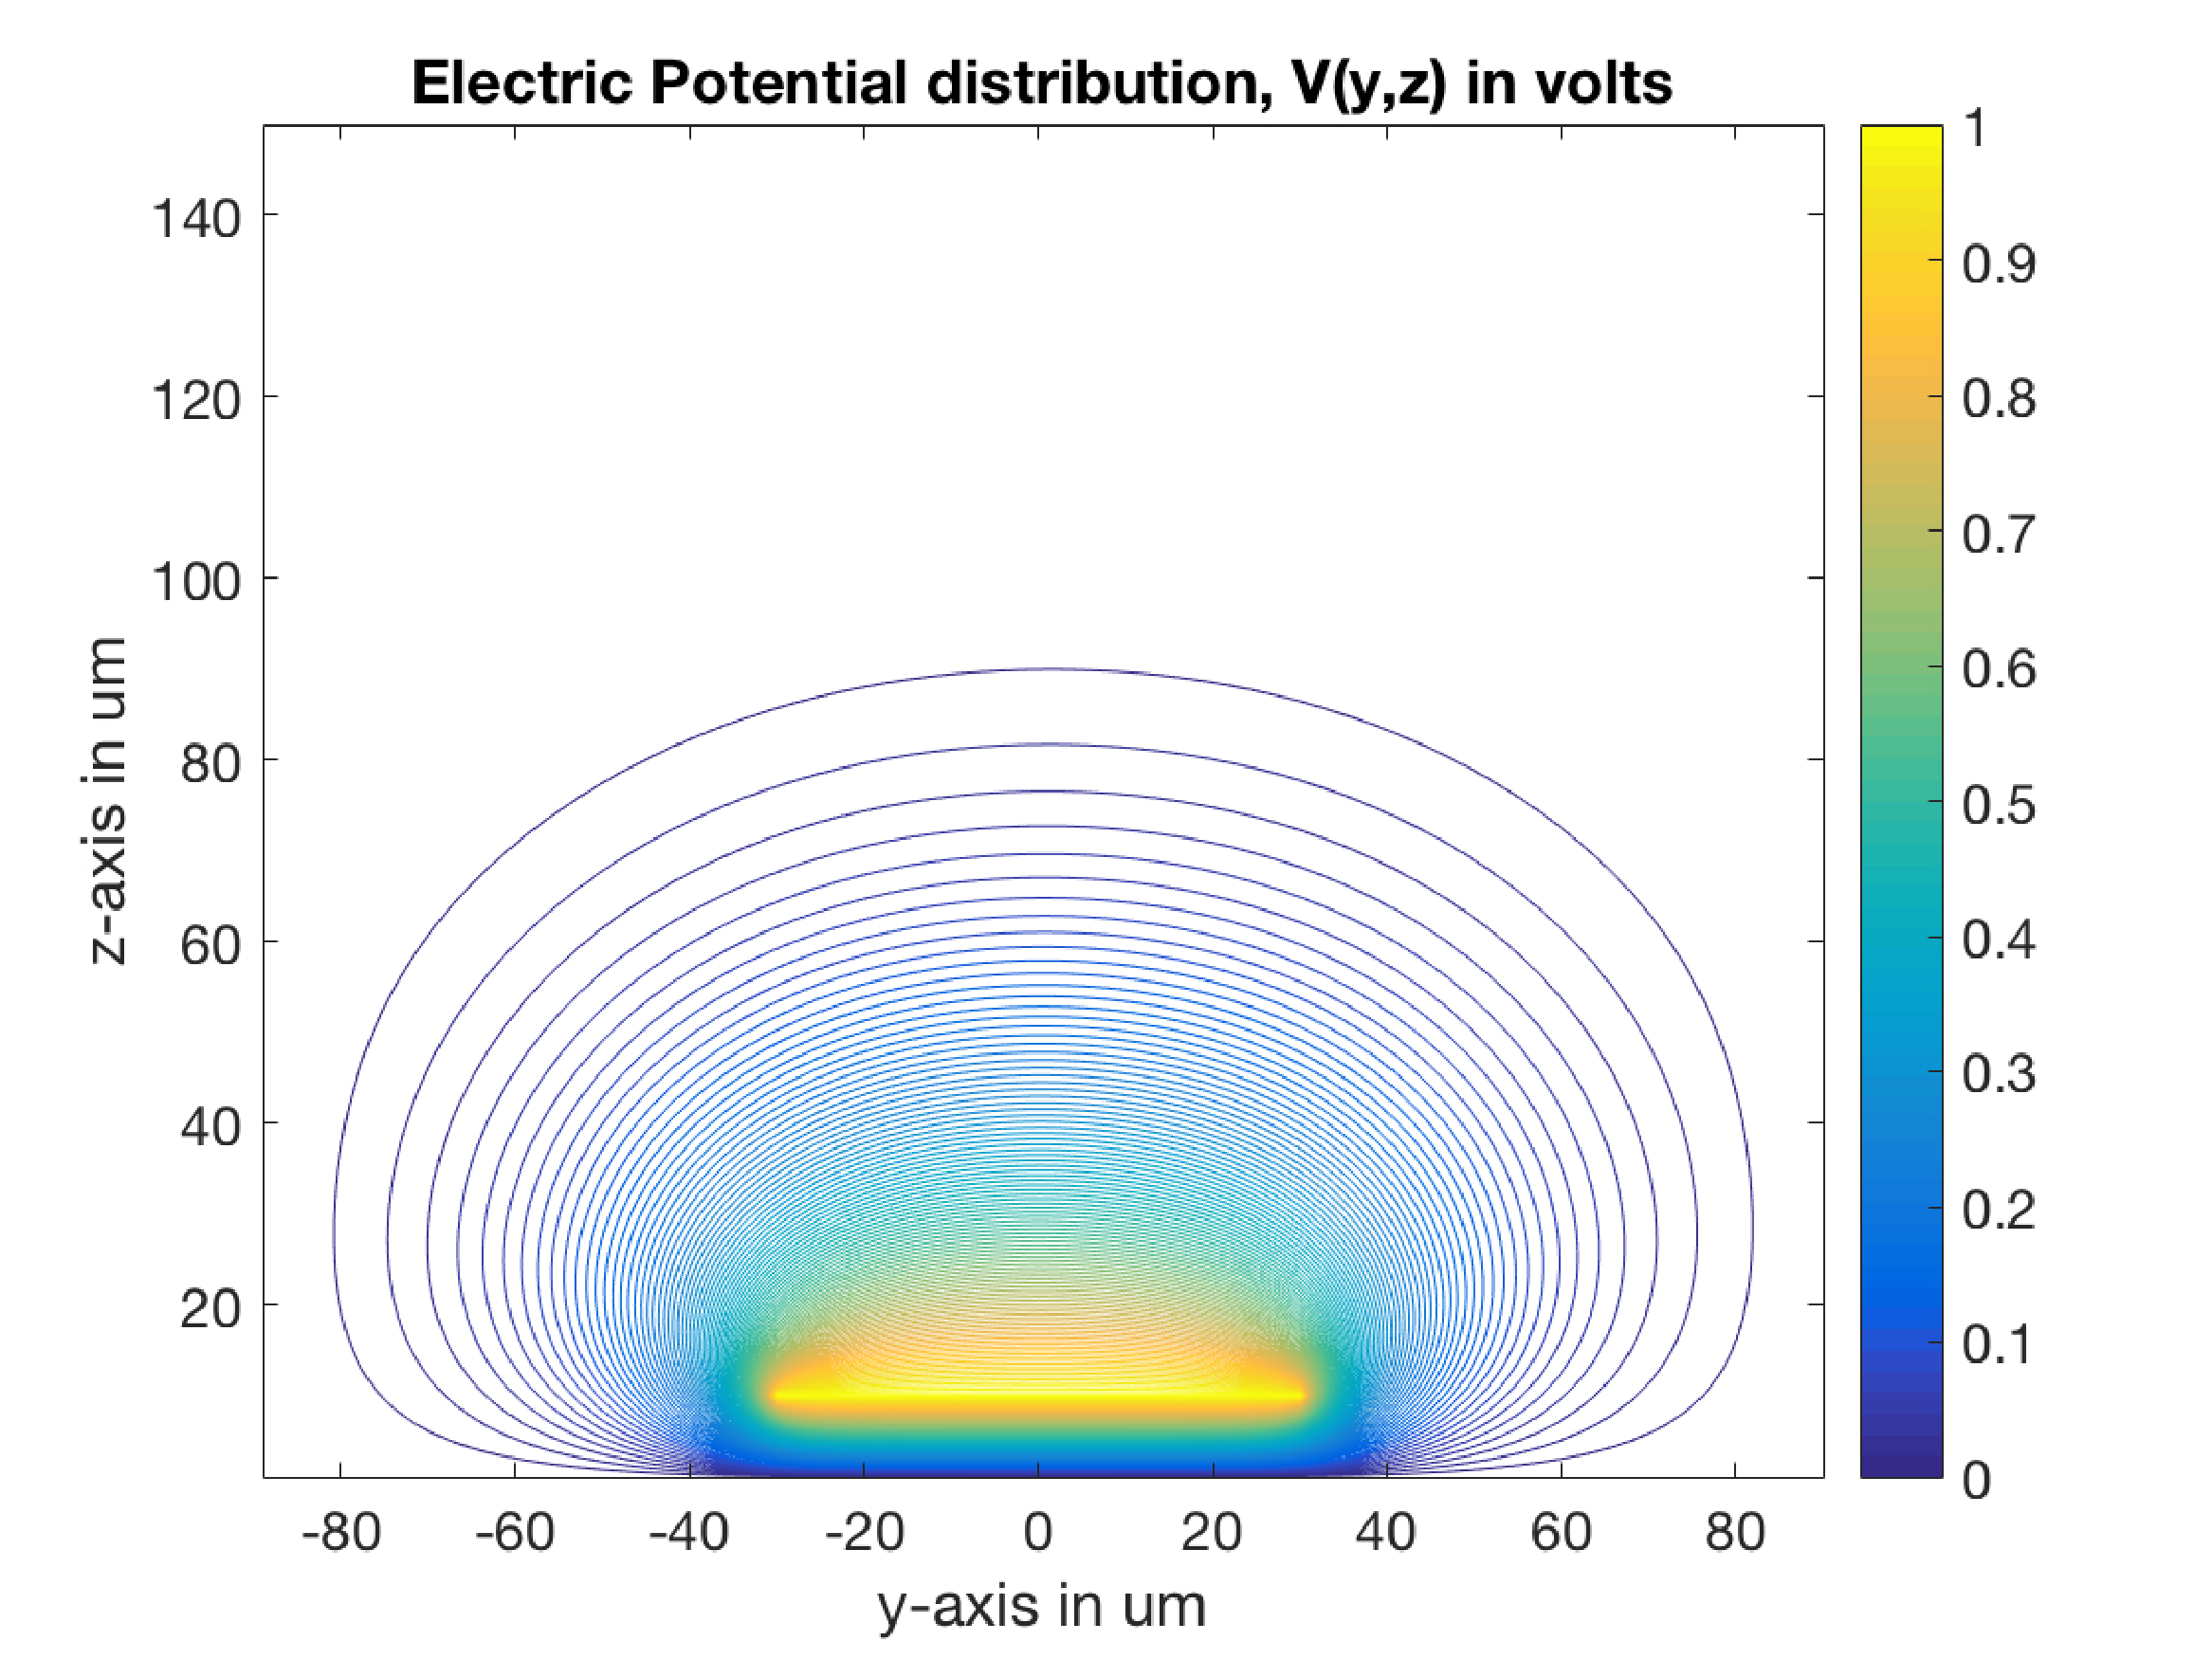
\includegraphics[scale=0.3]{images/TL_C.pdf}
\caption{Calculated electrical potential distribution V(y,z) with Matlab.}
\label{fig:TL_C}
\end{center}
\end{figure}

Subsequently, the electrical field can be calculated by $E=-\nabla \phi$ and then a arbitrary rectangular path was chosen to calculate its charge density $Q_{S}$ by integrating over the closed path. Finally, the distributed capacitance can be obtained with
 $C'=\frac{Q_{S}}{\phi}=9.31\times 10^{-10} F/m$.
\subsubsection{Distributed inductance}
After discretization, Eqn. (\ref{Eqn.:TL_L(2)}) can be expressed as
\begin{equation}
 \textbf{B}_{P}=\sum _{ i=1 }^{ n }{  \frac { \mu \textbf{I}\times { \textbf{r} }_{ i } \Delta y }{ 2\pi w{ r }_{ i}^{ 2 } }  }, \\
 \label{eq. TL_L}
 \end{equation}
 where, w is width of lateral cross section and $\textbf{r}$ is vector pointing from the surface element to the observation point P, $\mu$ is permeability depending on given medium and frequency. The magnetic field at each point on y-z plane can be solved as illustrated in Fig. \ref{fig:TL_L} by Matlab with "quiver" function. 

\begin{figure}[htbp]
\begin{center}
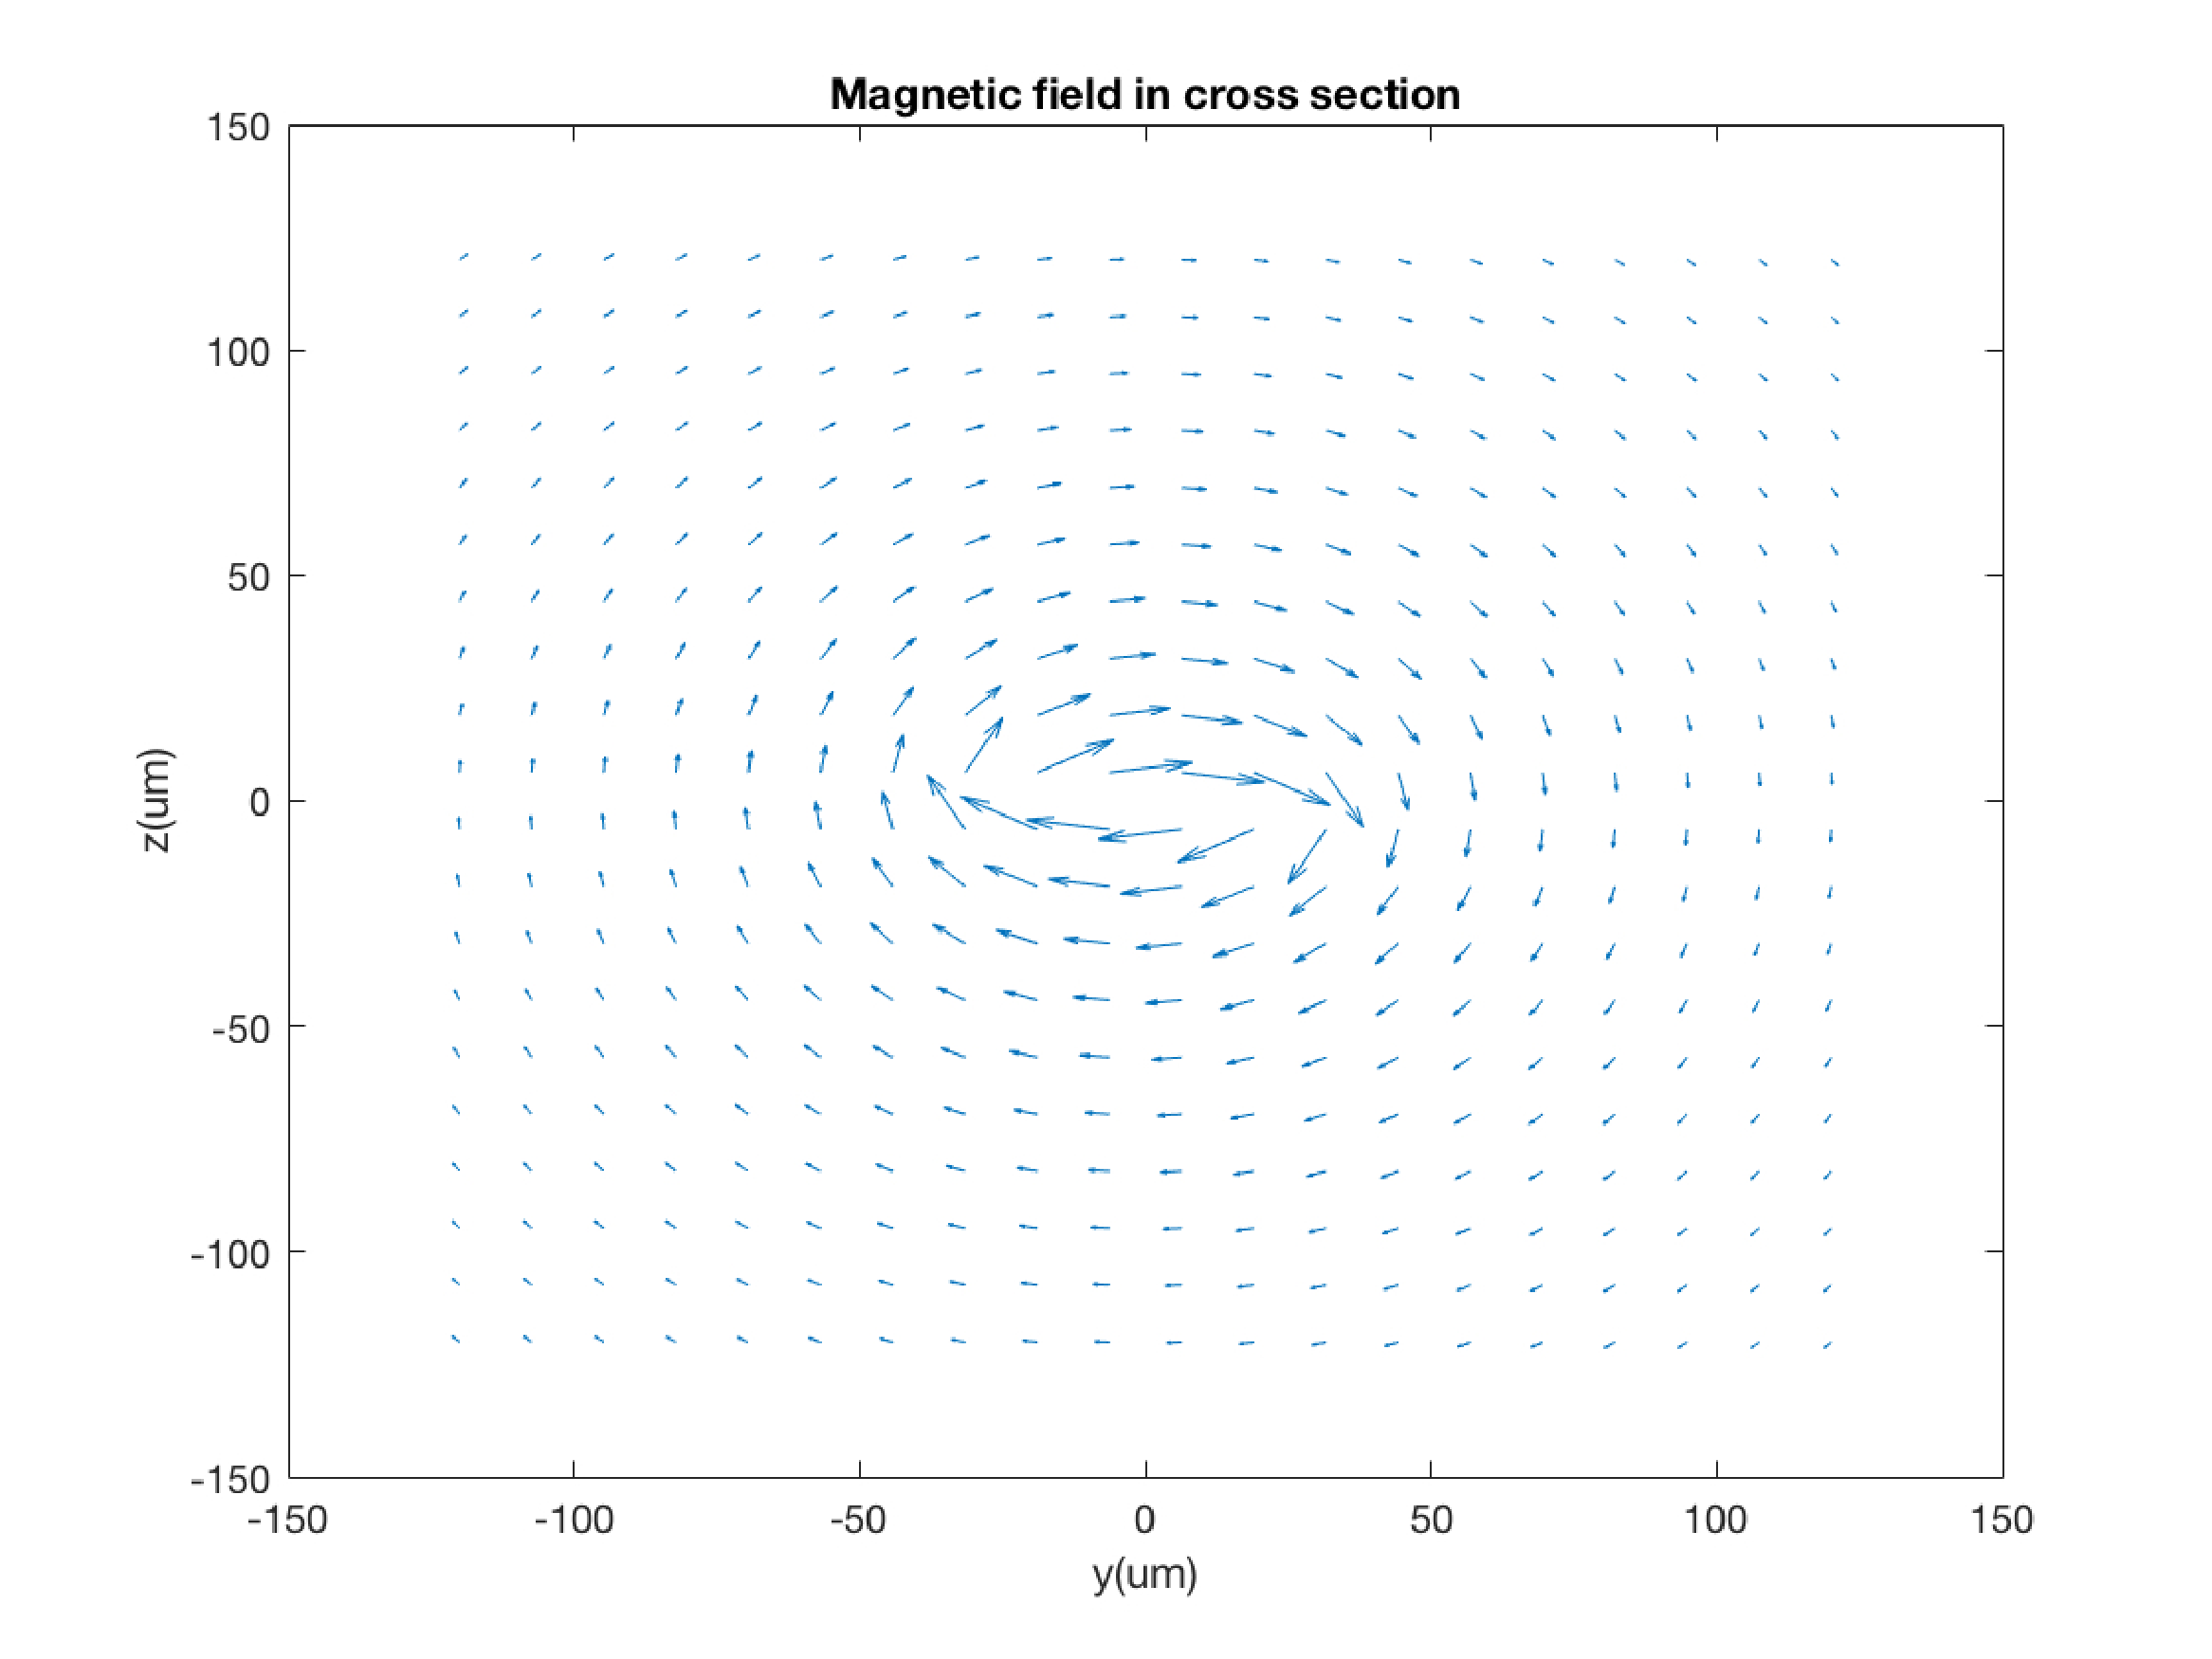
\includegraphics[scale=0.3]{images/TL_L.pdf}
\caption{Magnetic field in cross section (y-z plane) of QCL.}
\label{fig:TL_L}
\end{center}
\end{figure}
%
%\begin{equation}
%  W=\frac{1}{2}LI^{2}=\frac{1}{2}\underset { \Omega  }{\int }{ B H  } d\Omega
% \end{equation} 
% where $\textbf{H}$ is the auxiliary magnetic field and has a relation $\textbf{B}=\mu \textbf{H}$.
% 
Subsequently, the magnetic flux $\Phi$ can be calculated by integrating over a closed path, which is chosen with a arbitrary rectangular path for simplicity.  In active region, assuming $\mu\approx \mu_{0}$, then the distributed inductance can be obtained with $L'=\frac{\Phi }{I}=3.04\times 10^{-7} H/m$.
%
%    $L'=\frac{1}{c^{2}C'}=1.84\times 10^{-7} H/m$
%where c is the speed of light in vacuum.
 
\section{Modulation power}
Not only modulation frequency but also modulation power plays a key role in mode-locking. Even if QCL was modulated at near roundtrip frequency $f_{rt}$ , it can't be mode locked without enough modulation power. So it is essential to evaluate RF power for each simulation in order to analyze the modulation process. The RF source power can be easily calculated as modulation amplitude, signal function (since wave) as well as frequency are all known. But this power is total power and is larger than the power that was injected into QCL. Only the injected RF power will have influence on modulation.
%The reflection coefficient $\Gamma$ is defined as:
%\begin{equation}
%\Gamma = \frac{Z_{QCL}-Z_{S}}{Z_{QCL}+Z_{S}}
%\end{equation}

Two methods could be used to estimate modulation power:

1. Through Fourier Transformation ac component can be easily separated at modulation frequency $f_{RF}$ from recorded whole current data over time. Through its intensity fraction of dc component, the injected average RF current can be estimated. In the way, average applied RF voltage can also be obtained. Therefore, the injected RF-power to QCL is approximately:
\begin{equation}
 P_{RF}=\delta I* \delta V.
 \end{equation}
Where $\delta I$ and $ \delta V$ are current and voltage components with frequency of $f_{RF}$, respectively. They can be obtained by Fourier Transform of recorded data after simulation. The calculated value in this way should larger than realistic injected RF power, because even without RF source the laser itself has also current and voltage components with frequency of $f_{tr}$ due to microstrip line structure.

2. The impedance of transmission line (in this case QCL) at certain frequency is 
\begin{equation}
Z_{QCL}=\sqrt{\frac{R'+j2\pi f_{RF}L'}{G'+j2\pi f_{RF}C'}}.
\end{equation}
For calculation of small signal current modulation, there is a formula \cite{ramo2008fields} can be used 
\begin{equation}
{ P }_{ diss }=\frac { \delta { I }_{ QCL }^{ 2 }*Re[{ Z }_{ QCL }] }{ 2 }.
\end{equation}

Where $\delta { I }_{ QCL }$ is induced current variation due to RF source. The distributed conductance G' can be obtained through I-V characteristic curve of QCL.

Both of these two methods above were used to handle simulation data. The calculated RF power by them has quite small variation.

\chapter{Simulation Results}
The laser simulated in this work is based on doped $GaAs/Al_{x}Ga_{1-x}As$, which is 3 mm-long, 60 $\mu m$ wide, with height of 10 $\mu m$ metal-metal QCL. It is driven at 77 K and has an emission frequency of 3.8 THz. The average doping level of the active region is $5\times 10^{16} cm^{3}$. Its well and barrier widths are 4.6/9.8/2.6/9.0/4.4/17.6 nm. ???x?

\section{Simulation setup}
The simulation setup is illustrated in Fig. \ref{fig:schematicSETUP}. The QCL is biased by DC source and modulated by RF source. They are combined by bias-T and then connected with QCL through a wire with impedance $Z_{s}$. Both source are chose as voltage source for convenience. DC bias of QCL was set 8.6 kV/cm in this simulation work, which is a little higher than that at threshold voltage. 
\begin{figure}[htbp]
\begin{center}
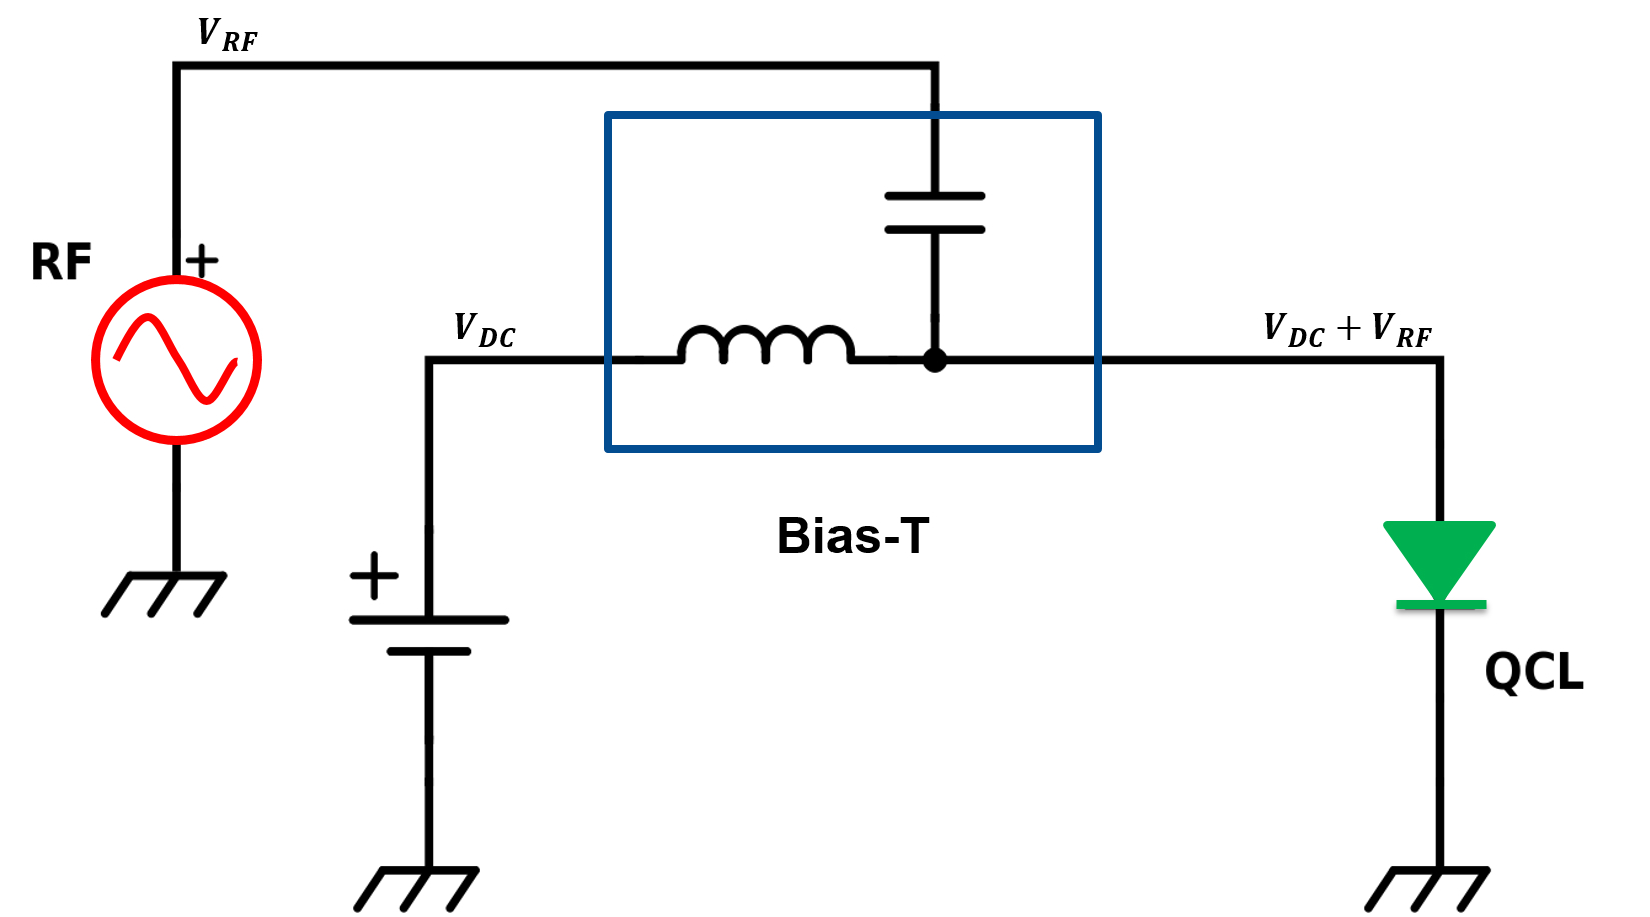
\includegraphics[scale=0.4]{images/schematicSETUP}
\caption{Schematic scheme of simulation setup. The green diode at at right side represents simulated QCL.}
\label{fig:schematicSETUP}
\end{center}
\end{figure}

\begin{table}[]
\centering
\caption{Simulation parameters}
\label{SIMparameter}
\begin{tabular}{llll}
\hline
\multicolumn{1}{|l|}{\textbf{Name}}  & \multicolumn{1}{l|}{\textbf{Symbol}} & \multicolumn{1}{l|}{\textbf{Value}} & \multicolumn{1}{l|}{\textbf{Unit}}         \\ \hline
\multicolumn{1}{|l|}{Cavity length}  & \multicolumn{1}{c|}{$L_{tot}$}       & \multicolumn{1}{c|}{3}              & \multicolumn{1}{c|}{mm}                    \\ %\hline
\multicolumn{1}{|l|}{Cavity height}  & \multicolumn{1}{c|}{$h$}       & \multicolumn{1}{c|}{10}              & \multicolumn{1}{c|}{um}                    \\ 

\multicolumn{1}{|l|}{Cavity width}  & \multicolumn{1}{c|}{$w$}   & \multicolumn{1}{c|}{60}              & \multicolumn{1}{c|}{um}                    \\ %\hline
\multicolumn{1}{|l|}{Doping density} & \multicolumn{1}{c|}{$D_{p}$ }        & \multicolumn{1}{c|}{1.5E16}         & \multicolumn{1}{c|}{$cm^{-3}$} 			   \\ %\hline
\multicolumn{1}{|l|}{Period length}  & \multicolumn{1}{c|}{$L_{p}$}         & \multicolumn{1}{c|}{50}           & \multicolumn{1}{c|}{nm}                    \\ %\hline
\multicolumn{1}{|l|}{Overlap factor} & \multicolumn{1}{c|}{$\Gamma$}          & \multicolumn{1}{c|}{0.8}          & \multicolumn{1}{c|}{}                      \\ 
 \multicolumn{1}{|l|}{Cavity loss}     &  \multicolumn{1}{c|}{$L_{\alpha}$}    &\multicolumn{1}{c|}{12}				&  \multicolumn{1}{c|}{$1/cm$} 						\\ \hline
\end{tabular}
\end{table}


\section{Results}
The amount of simulated iterations are 400 roundtrips, and during each simulation those important variables (e.g. optical field $E_{z}$, voltage, current, current density) at the middle point (x=L/2) of QCL were recorded after every time step.
\subsection{Characteristics of QCL}
Fig. \ref{fig:IVcurve} shows the voltage-current–luminance characteristics of the simulated QCL, which was obtained by supplying the QCL with a series of voltages ranging from 7.4 V to 10.8 V. The threshold voltage $V_{th}$ of the QCL is about 8.3 V, which means, under that there will be no lasing. Starting from $V_{th}$, the output emission will increase exponentially with higher voltage until tunneling phenomena occurs. At this area, QCL owns negative differential resistance (NDR) which is similar with tunneling diode. A large amount of injected electrons will directly pass active region through tunneling rather than transition from upper and lower laser levels accompanied with emission of photons. Therefore, the increasing input voltage will not contribute to laser output power. 

\begin{figure}[htbp]
\begin{center}
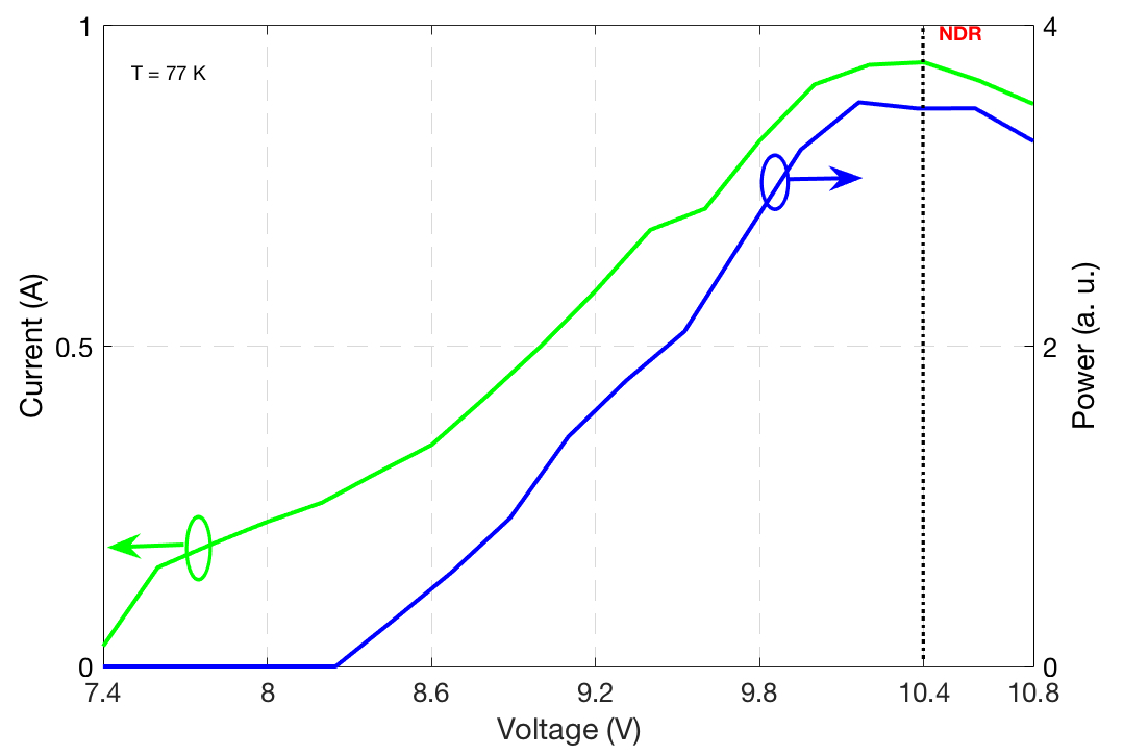
\includegraphics[scale=0.6]{images/IVCURVE.pdf}
\caption{voltage-current-luminance characteristics of simulated QCL.}
\label{fig:IVcurve}
\end{center}
\end{figure}

Besides, the roundtrip frequency of this QCL was obtained by Fourier transformation of both its optical field and electrical voltage. As Fig. \ref{fig:beatnote_noRF} shows the beatnote of simulated QCL without RF source, its roundtrip frequency $f_{rt}$ is about 13.34 GHz.
\begin{figure}[htbp]
\begin{center}
\includegraphics[scale=0.8]{images/Beatnote_noRF.pdf}
\caption{Beatnote of the simulated QCL without RF source. Its roundtrip frequency $f_{rt}$ is about 13.34 GHz.}
\label{fig:beatnote_noRF}
\end{center}
\end{figure}

\subsection{Modulation with RF source} 
A series of simulations were carried out for investigating the influence of modulation power as well frequency on mode-locking of QCLs. After 400 roundtrips simulation, pulse train was clearly observed.
% as Figure \ref{fig:FWHM} shows, from 4610 to 4690 ps in corresponding to 164 roundtrip time $T_{rt}$. Its Full Width at Half Maximum (FWHM) in this modeling is around 11.6 ps, which shows quite good agreement with experiment result 11 ps \cite{gellie2010injection}.
%\begin{figure}[htbp]
%\begin{center}
%\includegraphics[scale=0.6]{images/FWHM.eps}
%\caption{Singel pulse from simulation.}
%\label{fig:FWHM}
%\end{center}
%\end{figure}

Before simulation was carried out, firstly two parameters ($M_{A}$ and $f_{RF}$) have to be roughly defined. Although the function of RF source is known with $V_{RF}^{n}=M_{A}\cos(2\pi f_{RF}n\Delta t)$ and its power is proportional to square of its amplitude $M_{A}$, the injected power to QCL can still not be determined before simulation. Due to reflection as well as attenuation on wire between RF source and QCL, the injected power should be smaller than the power coming from RF source. But it is well known that theoretically optimal modulation frequency should exactly at roundtrip frequency. Therefore, simulations with different power and certain $f_{RF}$ were firstly carried out.
\subsubsection{Modulation with different power} 
Lack of sufficient modulation power, QCLs can still not be mode-locked even if modulation frequency is equal to $f_{rt}$. Therefore, modulations with different RF amplitude ($M_{A}$) was investigated, in which they all have the same modulation frequency and all the other parameters are the same as well. With increasing modulation power the side modes around main mode were strengthened (See Fig. \ref{fig:modA_Beatnote}) and will contribute to generate ultra short pulse. The bandwidth of frequency spectra was increasing consequently from 40 GHz to larger than 100 GHz. The optical field was mode-locked at modulation frequency $f_{RF}$, which is set at 13.9 GHz and a little higher than roundtrip frequency of this laser. 
%\begin{figure}[htbp]
%\begin{center}
%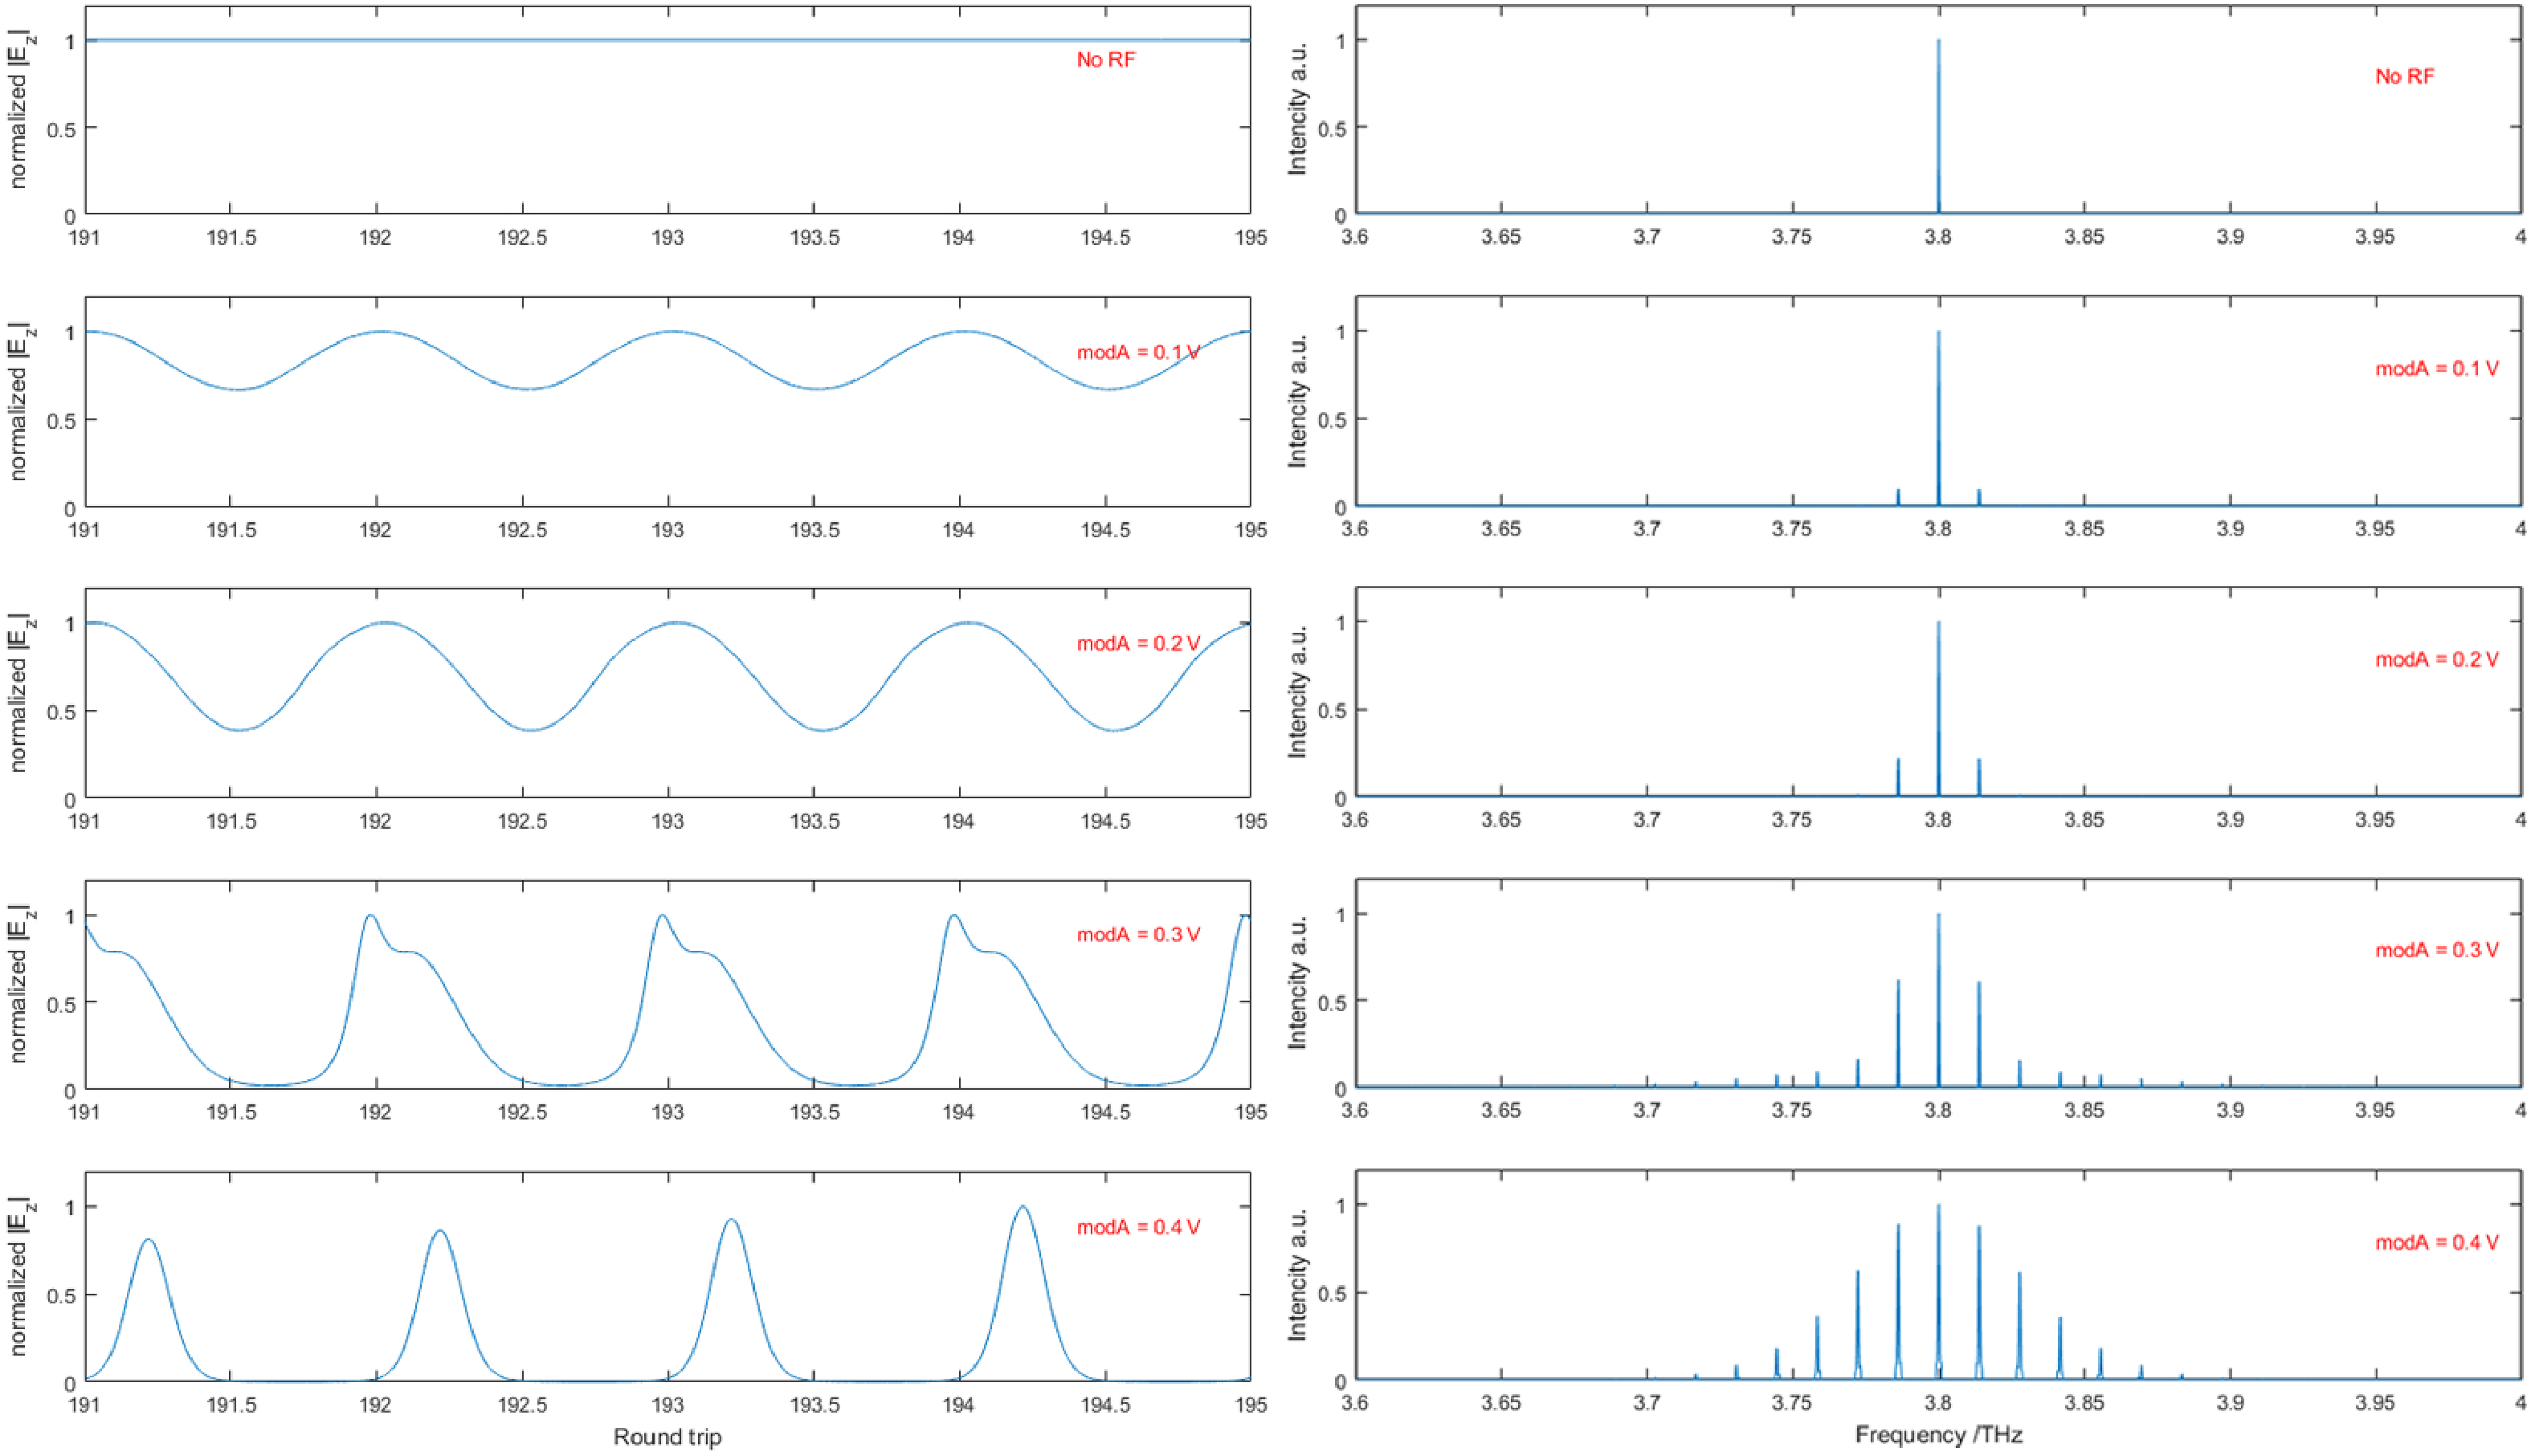
\includegraphics[scale=0.28]{images/modA_spectra.pdf}
%\caption{Normalized spectra in time as well as frequency domain with different modulation powers. modA denotes RF amplitude. $f_{RF}$ of RF source is at roundtrip frequency and QCL is bias by 8.6 kV/cm}
%\label{fig:modA_fspectra}
%\end{center}
%\end{figure}
\begin{figure*}[htbp]
  \centering
  \subfigure[]{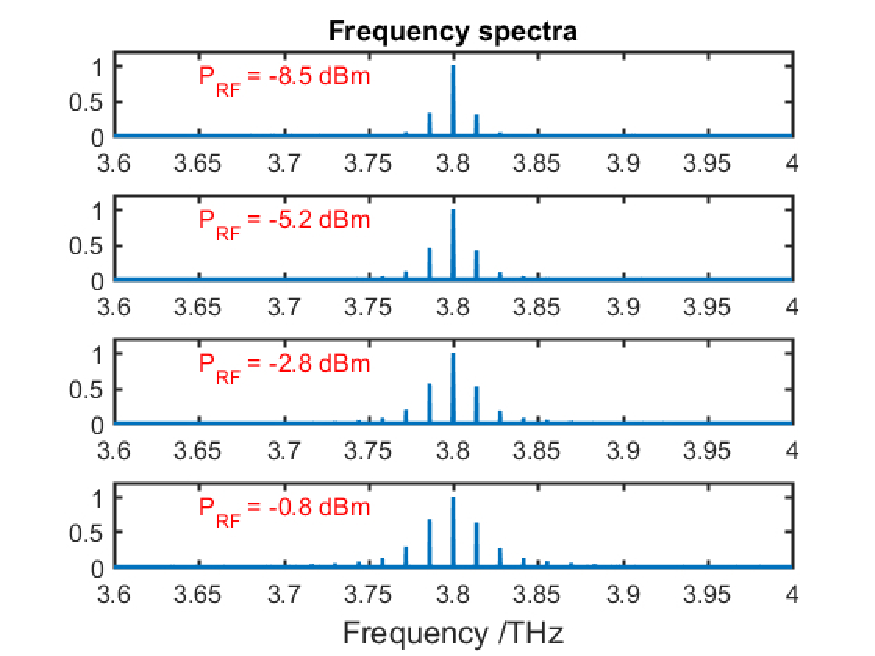
\includegraphics[scale=0.9]{images/fa.pdf}}
  \subfigure[]{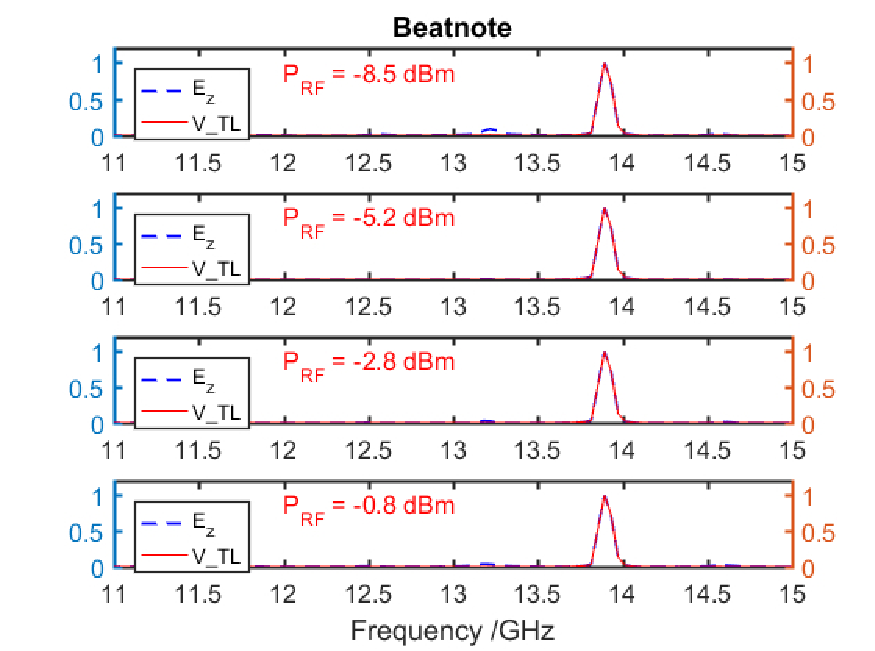
\includegraphics[scale=0.9]{images/Ba.pdf}}
\caption{(a)Frequency spectra of QCL emission with increasing modulation power from -8.5 dBm to -0.8 dBm. The simulated QCL has optical emission frequency of 3.8 THz. (b) Beatnote of optical field $E_{z}$ (dashed blue line) and electrical voltage $V\_{TL}$ (red solid line).}
\label{fig:modA_Beatnote}
\end{figure*}

Fig. \ref{fig:Pulse_modA} shows their corresponding emission pulses at time domain with increasing injected RF power. The time axis was normalized in roundtrips (from 391 to 396 roundtrips) and intensity was normalized by the maximum of all cased. Hence, they can be easily compared in terms of both pulse duration and emission power. Full Width at Half Maximum (FWHM) was used for quantifying their pulse duration. As illustrated in Fig. \ref{fig:Pulse_modA}, the more RF power was injected, the shorter emission pulse of QCL shows. Also with higher injected RF power, QCL has larger emission power. The emission intensity with RF power -0.8 dBm is twice larger the same as that with RF power -8.5 dBm.
\begin{figure}[htbp]
\begin{center}
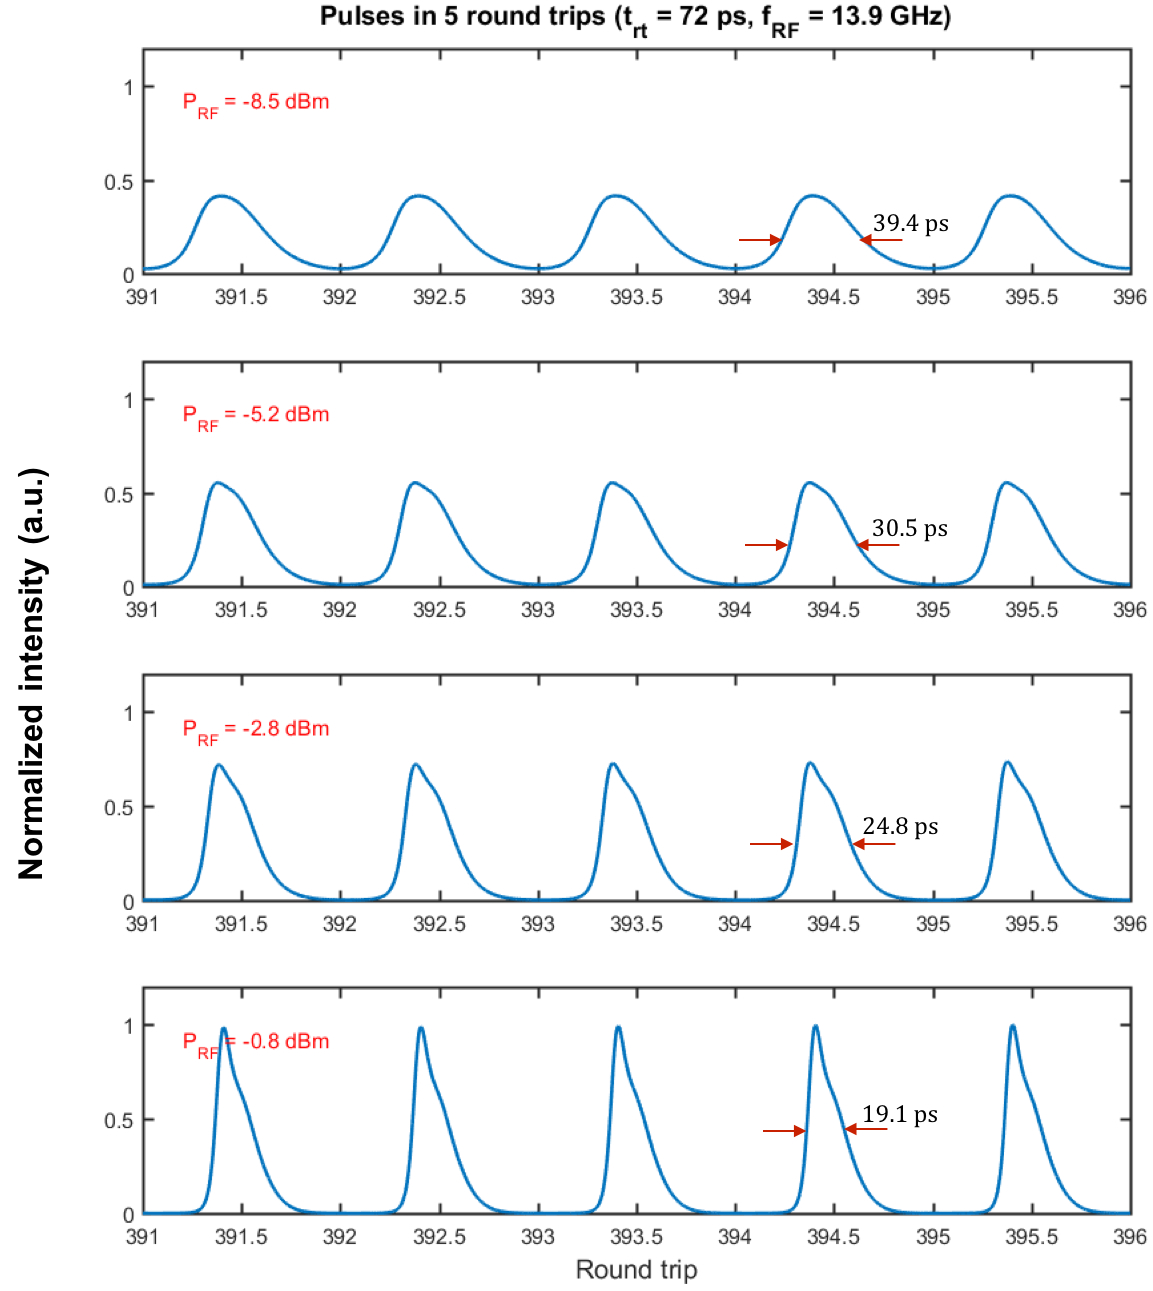
\includegraphics[scale=0.5]{images/Pulse_modA.pdf}
\caption{Pulse trains in five roundtrips, in which their emission intensity were normalized by the highest intensity among all cases.}
\label{fig:Pulse_modA}
\end{center}
\end{figure}

\subsubsection{Modulation with different frequencies} 
Modulation frequency is a key factor for mode-locking. As already discussed at chapter 2.3 Mode-locking, the modulation frequency has to be close to roundtrip frequency. To investigate its maximal possible locking range, the laser was modulated with a large frequency interval nearby $f_{rt}$ and the modulation amplitude $M_{A}$ was fixed with 6 V, all the other parameters remain the same.

Similar with in modulation with different powers, frequency spectra and beatnote were used to check the influence and whether mode-locking was achieved. If no RF source exists, QCL emits continuous light as expected and will show a clear single peak in frequency domain (See Fig. \ref{fig:modA_Beatnote}), which is at its emission frequency (in this case 3.8 THz). With increasing modulation frequency, the bandwidth of their frequency spectra were also increased and optical field was mode-locked at $f_{RF}$.
\begin{figure*}[htbp]
  \centering
  \subfigure[]{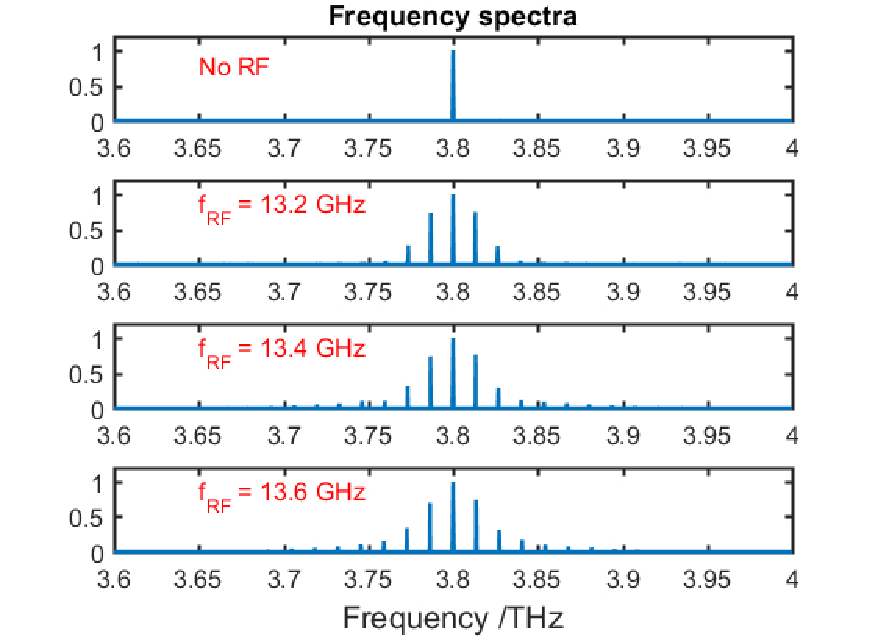
\includegraphics[scale=0.9]{images/f.pdf}}
  \subfigure[]{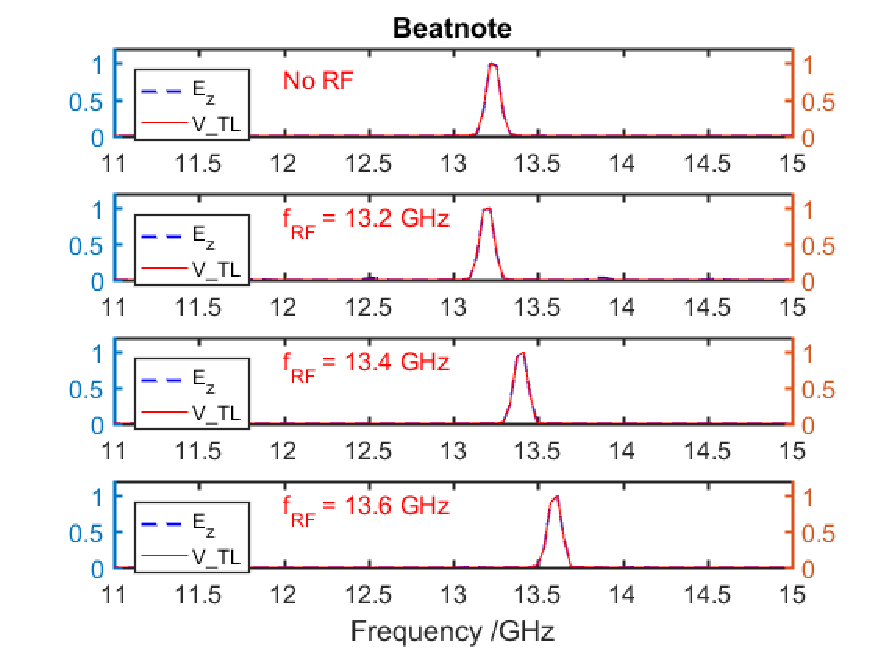
\includegraphics[scale=0.9]{images/B.pdf}}
\caption{(a)Frequency spectra of QCL emission with increasing modulation frequency from -8.5 dBm to -0.8 dBm. The simulated QCL has optical emission frequency of 3.8 THz. (b) Beatnote of optical field $E_{z}$ (dashed blue line) and electrical voltage $V\_{TL}$ (red solid line).}
\label{fig:modA_Beatnote}
\end{figure*}

To check their corresponding pulse shapes in each case, 5 roundtrips was chosen with various modulation frequencies ranging from 13 GHz to 14.9 GHz illustrated in Fig. \ref{fig:Pulse_modF}. Also their emission intensity (proportional to $|E_{z}^{2}|$ ) were normalized to the one which has highest intensity for comparison.  The shortest pulses were found at modulation frequency 13.6 GHz, which have FWHM of 17.2 ps. However, after calculation of their realistic injected RF power, it can be found that the powers injected in all case have small variation rather than the same, although each has the same modulation amplitude. This can be explained because QCL is not a lumped element like resistor, its characteristics can be affected by both electrical and optical field.

Moreover, by comparing the bottom three cases which have RF source (See Fig. \ref{fig:Pulse_modF}), it was found that the increasing modulation frequency and injected RF power will not always contributed to generate ultra short pulse. From $f_{RF}$=13.2 GHz to 13.4 GHz, the pulse becomes wider, FWHM increases from 22.2 ps to 24.5 ps correspondingly, although the injected power into QCL was increased slightly. That's also the reason why we do need to presume appropriate simulation model, which will help experiments a lot to generate short pulse with smallest modulation power as possible.
\begin{figure}[htbp]
\begin{center}
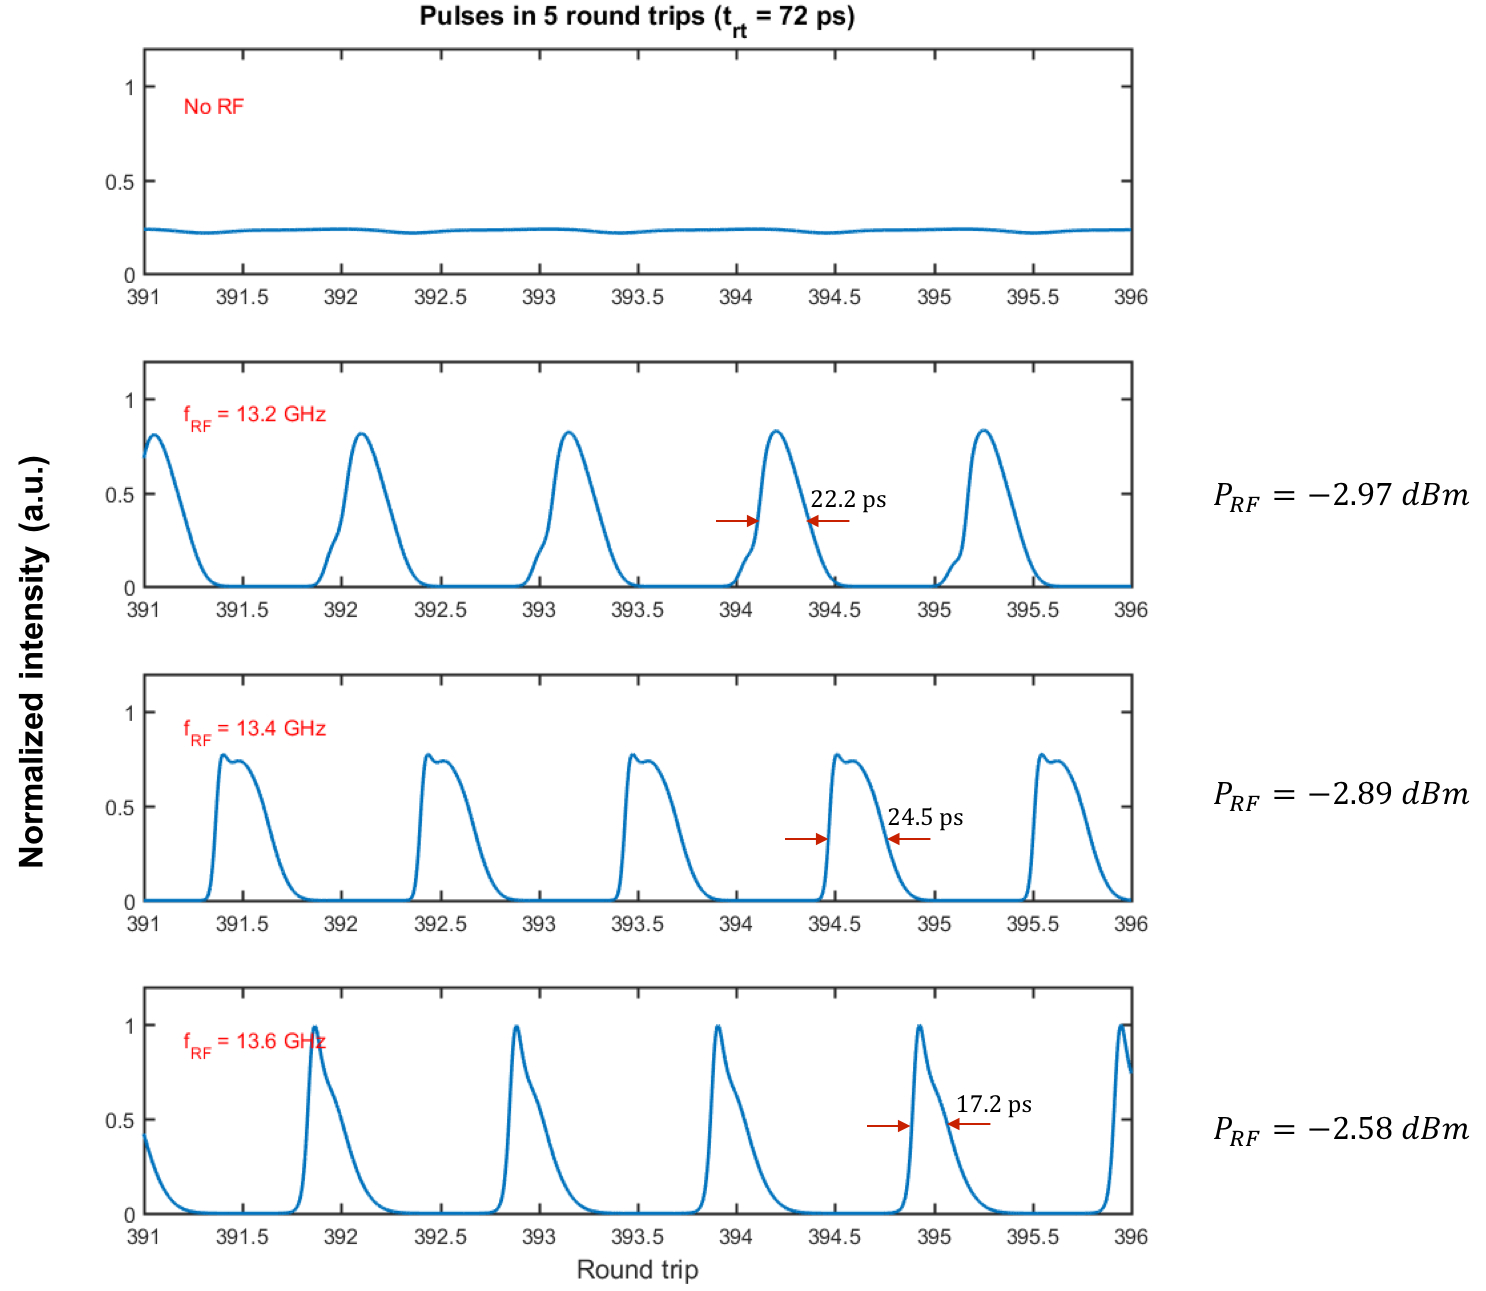
\includegraphics[scale=0.5]{images/Pulse_modF.pdf}
\caption{Pulse trains in five roundtrips, and their emission intensity were normalized by the highest intensity among all cases. The first case was without RF source and the left were modulated with same amplitude $M_{A} = 6 V$. Their corresponding injected RF powers were shown at right side after each case.}
\label{fig:Pulse_modF}
\end{center}
\end{figure}

\section{Comparison with experiment}
Compared with experiment results from Ref. \cite{wang2015generating}, which used the same QCL as in this work, the voltage-current-luminance curve shape has good agreement with that measured in experiment except for the quite larger kink area. The obtained shortest pulse in this modeling has FWHM of 17.2 ps while in experiment \cite{wang2015generating} is 11 ps (See Fig. \ref{fig:comparison}). Besides, similar pulse shape was observed. However, due to the restriction of optical modeling, the operating power of this QCL (about 2.4 W) is quite small compared with in experiment (about 10 W). With same injected RF power, it will be more easily mode-locked because the locking-band width is inversely proportional to square root of free-running oscillator power \cite{gellie2010injection}. Therefore, "pulling effect" in beatnote was also not observed in this simulation and locking range can also not be determined.


\begin{figure}[htbp]
\begin{center}
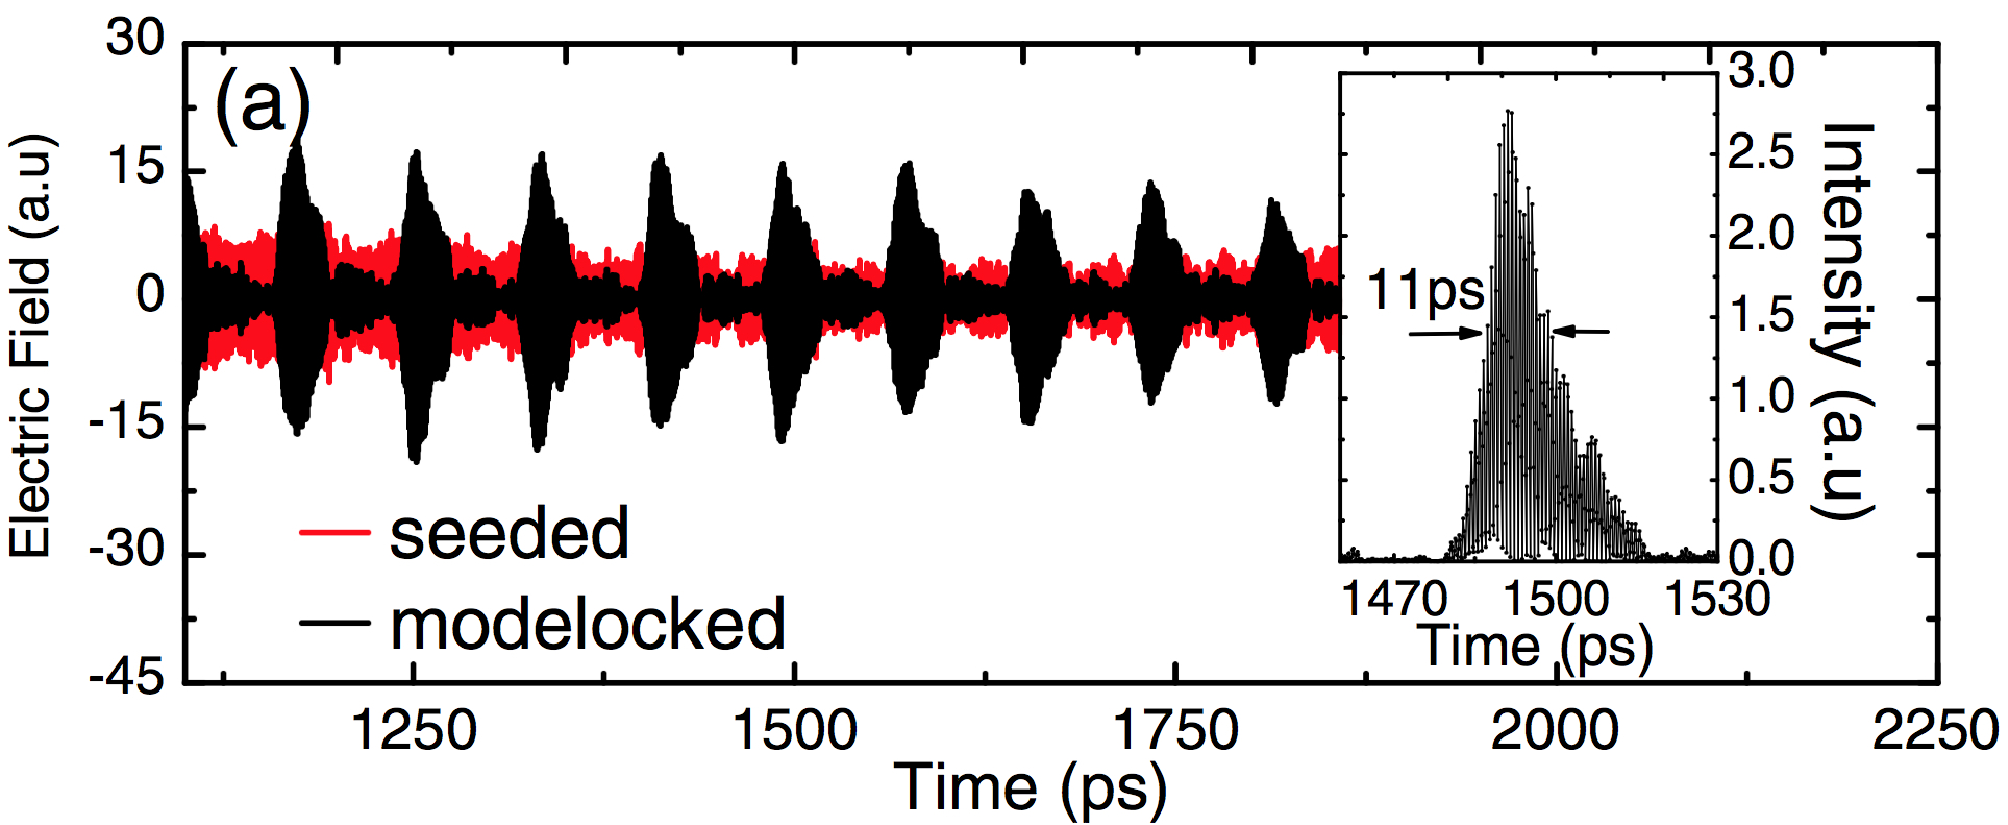
\includegraphics[scale=0.4]{images/comparison.pdf}
\caption{Experiment data from Ref. \cite{wang2015generating}: output electric field for the seeded (red) and mode-locked (black) QCLs with an applied microwave modulation of 12.46 GHz for the latter. Inset: expanded view of the THz pulse intensity between 1470 and 1530 ps. }
\label{fig:comparison}
\end{center}
\end{figure}
\chapter{Conclusion}
In this work a dynamic model was build, which is based on Maxwell-Bloch equations and Transmission line for electro-optical simulations of QCLs. Different with pure optical simulations, electrical behavior was also taken into consideration in this model. The applied voltage signal propagates along cavity in the direction of propagation and also has nature of wave. Due to similar topology with microstrip transmission line, Transmission line method was introduced for this modeling, which helps to study of electrical behavior. Both electrical modeling (Transmission line approach) and optical modeling (Maxwell-Bloch equations) were simulated simultaneously and worked well with each other. 

Through this model active mode-locking of THz QCL was intensively investigated. A series of simulations were carried out with different modulation parameters. During simulation mode-locking was achieved and it was found pulse duration can be largely affected by injected RF power as well as modulation frequency. Moreover, short pulse with FWHM of 17.2 ps was observed in this work and its pulse shape has good agreement with that from experiment.


% -----------------------------
%   LITERATUR VERZEICHNIS
% -----------------------------

%\addcontentsline{toc}{chapter}{List of Figures}
%\listoffigures

\renewcommand*{\bibname}{Bibliography} % Using "Sources" as the title of the section
\bibliography{reference}{}
\addcontentsline{toc}{chapter}{Bibliography}

\bibliographystyle{ieeetr}

\end{document}
